%!TEX program = xelatex
\documentclass[UTF8]{ctexart}

% math bracket
%  ()
\newcommand{\brc}[1]{\left({{}#1}\right)}
%  []
\newcommand{\brm}[1]{\left[{{}#1}\right]}
%  ||
\newcommand{\brv}[1]{\left|{{}#1}\right|}
%  {}
\newcommand{\brf}[1]{\left\{{{}#1}\right\}}
%  ||
\newcommand{\brt}[1]{\left\Vert{{}#1}\right\Vert}
%  <>
\newcommand{\brg}[1]{\left<{{}#1}\right>}
%  floor
\newcommand{\floor}[1]{\lfloor{{}#1}\rfloor}
%  ceil
\newcommand{\ceil}[1]{\lceil{{}#1}\rceil}

% font
\newcommand{\fira}[1]{{\firacode {}#1}}

% abbr command
\newcommand{\ds}{\displaystyle}
\newcommand{\pt}{\partial}
\newcommand{\rint}[2]{\Big|^{{}#1}_{{}#2}}
\newcommand{\leg}{\left\lgroup}
\newcommand{\rig}{\right\rgroup}

% math symbol
\newcommand{\de}{\mathrm{d}}
\newcommand{\im}{\mathrm{im}}
\newcommand{\ord}{\mathrm{ord}}
\newcommand{\cov}{\mathrm{Cov}}
\newcommand{\lub}{\mathrm{LUB}}
\newcommand{\glb}{\mathrm{GLB}}
\newcommand{\var}{\mathrm{Var}}
\newcommand{\aut}{\mathrm{Aut}}
\newcommand{\sylow}{\mathrm{Sylow}}
\newcommand{\xhi}{\mathcal{X}}
\newcommand{\po}{\mathcal{P}}
\newcommand{\bi}{\mathrm{b}}
\newcommand{\rfl}{\mathcal{R}}

% algorithmic symbol
\newcommand{\gro}{\mathrm{O}}

\newfontfamily\firacode{Fira Code}
\newfontfamily\mincho{MS Mincho}

% math
\usepackage{ntheorem}
\usepackage{ulem}

\theoremseparator{ }
\newtheorem{dft}{Definition}
\newtheorem{tem}[dft]{Theorem}
\newtheorem{lem}[dft]{Lemma}
\newtheorem{epe}[dft]{Example}
\newtheorem{cor}[dft]{Corollary}

\usepackage{mathrsfs}
\usepackage{amsmath}
\usepackage{amssymb}
\usepackage{cancel}
%\usepackage{amsthm}

% control
\usepackage{ifthen}
\usepackage{intcalc}
\usepackage{array}

% format
\usepackage{indentfirst}
\usepackage{enumerate}
\usepackage{url}
\usepackage{setspace}

\usepackage{xcolor}

\definecolor{ballblue}{rgb}{0.13, 0.67, 0.8}
\definecolor{celestialblue}{rgb}{0.29, 0.59, 0.82}
\definecolor{bananayellow}{rgb}{1.0, 0.88, 0.21}
\definecolor{brilliantlavender}{rgb}{0.96, 0.73, 1.0}
\definecolor{burgundy}{rgb}{0.5, 0.0, 0.13}
\definecolor{cadmiumorange}{rgb}{0.93, 0.53, 0.18}
\definecolor{aqua}{rgb}{0.0, 1.0, 1.0}
\definecolor{auburn}{rgb}{0.43, 0.21, 0.1}
\definecolor{brass}{rgb}{0.71, 0.65, 0.26}
\definecolor{tangerine}{rgb}{0.95, 0.52, 0.0}
\definecolor{portlandorange}{rgb}{1.0, 0.35, 0.21}
\definecolor{mediumred-violet}{rgb}{0.73, 0.2, 0.52}

% listing set
\definecolor{func}{rgb}{0.29, 0.59, 0.82}
\definecolor{ftype}{rgb}{0.95, 0.52, 0.0}
\definecolor{cls}{rgb}{1.0, 0.35, 0.21}
\definecolor{slf}{rgb}{0.73, 0.2, 0.52}
\definecolor{backg}{HTML}{F7F7F7}
\definecolor{str}{HTML}{228B22}
% attestation
\definecolor{atte}{RGB}{178,34,34}

\usepackage{listings}

\lstset{
    backgroundcolor = \color{backg},
    basicstyle = \small,%
    escapeinside = ``,%
    keywordstyle = \color{func},% \underbar,%
    identifierstyle = {},%
    commentstyle = \color{blue},%
    stringstyle = \color{str}\ttfamily,%
    %labelstyle = \tiny,%
    extendedchars = false,%
    linewidth = \textwidth,%
}

\usepackage{geometry}

\geometry{
    left=2.0cm,
    right=2.0cm,
    top=2.5cm,
    bottom=2.5cm
}

\usepackage[
    colorlinks,
    linkcolor=blue,
    anchorcolor=blue,
    citecolor=blue
]{hyperref}

% table
\usepackage{csvsimple}
\usepackage{multirow}

% graph
\usepackage{tikz}
\usepackage{pgfplots}
\usetikzlibrary{
    quotes,
    angles,
    matrix,
    arrows,
    automata
}


\title{自制操作系统-准备篇}
\author{向阳曦\ 2017211279\ 2017211301}
\date{}

\begin{document}
\setlength{\parindent}{2em}
%\renewcommand{\baselinestretch}{1.5}
\setlength{\baselineskip}{2.5em}
\maketitle
\section{课题硬件环境描述}

\begin{enumerate}[1]
	\item 硬件: TEC-8实验电路
	\begin{enumerate}[1]
		\item 74181ALU等
		\item 可编程逻辑芯片EPM7128
	\end{enumerate}
	\item 软件: Quartus II 9.0
\end{enumerate}

\section{题目分析}
\subsection{实验目标}

\begin{enumerate}[1]
	\item 完成硬连线控制器基础设计
	\item 在原指令的基础上扩指至少三条
	\item 修改PC指针功能
	\item 完成流水硬连线控制器基础设计
	\item 在原指令的基础上扩指至少三条
	\item 修改PC指针功能
\end{enumerate}

\subsection{设计思路}

\begin{enumerate}[1]
	\item 画出硬连线控制器运行流程图
	\item 将硬连线控制器运行流程图翻译成硬连线信号
	\item 将硬连线信号翻译成VHDL多分支程序
\end{enumerate}

\section{团队分工}
向阳曦负责程序指令翻译, 张逸群负责控制台程序.\\
报告方面,向阳曦主要完成tex矢量图绘画.两人一起完成指令解释.\\
\indent 合并一起以后,两人一起完成控制器程序的测试.
\section{设计详解}
\subsection{硬连线控制器}
硬连线控制器的关键是将$\mu \text{P}$(IR)信号作为控制信号的一部分,根据控制信号的组合逻辑完成下地址转移.\\
\indent 为了设计的方便,一般先将指令周期流程图画出,然后根据指令周期流程图写出组合逻辑.VHDL可以根据组合逻辑的特征,合并多个相似的控制信号组合为分支条件语句.
\subsubsection{硬连线控制器控制台指令流程图}
\begin{figure}[!h]
    \centering
    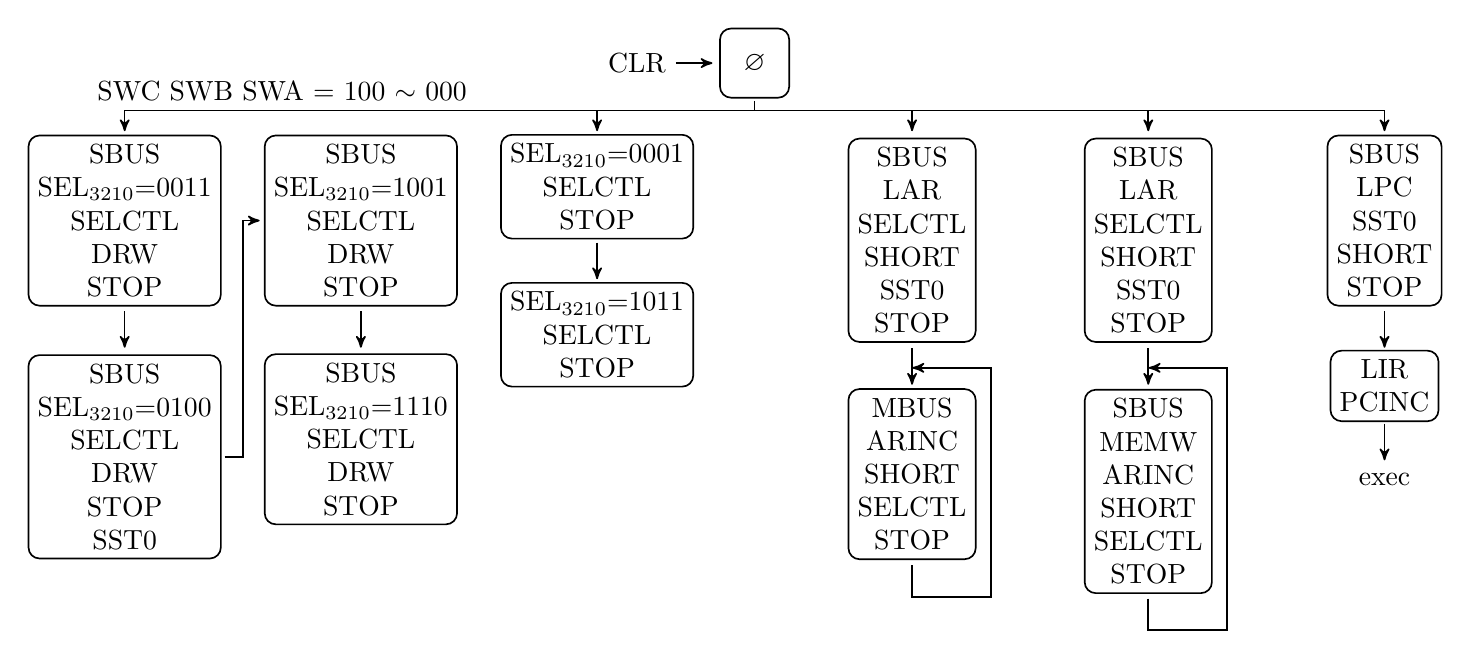
\begin{tikzpicture}[->,>=stealth',shorten >=1pt,auto,node distance=2.8cm,semithick]
    \tikzstyle{every state}=[shape=rectangle, rounded corners]
	\node[left] (clr) at (-1, 0) {CLR}; 
	\draw [->] (-1, 0) -- (-0.5,0);
	\node[state] (A) at (0, 0) {$\varnothing$};
	\node[state, align=center] (readra) at ( -8, -2) {SBUS\\ $\text{SEL}_{3210}$=0011\\ SELCTL\\ DRW\\ STOP};
	
	\node[state, align=center] (readrb) at ( -5, -2) {SBUS\\ $\text{SEL}_{3210}$=1001\\ SELCTL\\ DRW\\ STOP};

	\node[state, align=center] (readrc) at ( -8, -5) {SBUS\\ $\text{SEL}_{3210}$=0100\\ SELCTL\\ DRW\\ STOP\\ SST0};

	\node[state, align=center] (readrd) at ( -5, -4.777 ) {SBUS\\ $\text{SEL}_{3210}$=1110\\ SELCTL\\ DRW\\ STOP};
	
	\node[state, align=center] (readrd) at ( -2, -1.57 ) {$\text{SEL}_{3210}$=0001\\ SELCTL\\ STOP};
	\node[state, align=center] (readrd) at ( -2, -3.45 ) {$\text{SEL}_{3210}$=1011\\ SELCTL\\ STOP};

	\node[state, align=center] (readrd) at ( 2, -2.25 ) {SBUS\\ LAR\\ SELCTL\\ SHORT \\ SST0\\ STOP};
	\node[state, align=center] (readrd) at ( 2, -5.22 ) {MBUS\\ ARINC\\ SHORT\\ SELCTL\\ STOP};

	\node[state, align=center] (readrd) at ( 5, -2.25 ) {SBUS\\ LAR\\ SELCTL\\ SHORT \\ SST0\\ STOP};
	\node[state, align=center] (readrd) at ( 5, -5.44 ) {SBUS\\ MEMW\\ ARINC\\ SHORT\\ SELCTL\\ STOP};

	\node[state, align=center] (readrd) at ( 8, -2 ) {SBUS\\ LPC\\ SST0\\ SHORT\\ STOP};
	\node[state, align=center] (readrd) at ( 8, -4.10 ) {LIR \\ PCINC};
	%\path (A) edge[bend left] (B)
	\draw [->] (0, -0.48) -- (0, -0.6) -- (-8, -0.6) -- (-8, -0.9);
	\draw [->] (-8, -3.15) -- (-8, -3.65);
	\draw [->] (-6.73, -5) -- (-6.5, -5) -- (-6.5, -2) -- (-6.25, -2);
	\draw [->] (-5, -3.15) -- (-5, -3.65);

	\draw [->] (-2, -0.6) -- (-2, -0.9);
	\draw [->] (-2, -2.28) -- (-2, -2.78);

	\draw [->] (0, -0.6) -- (2, -0.6)-- (2, -0.9);
	\draw [->] (2, -3.62) -- (2, -4.12);
	\draw [->] (2, -6.38) -- (2, -6.78) -- (3, -6.78) -- (3, -3.87) -- ( 1.97, -3.87);
	\draw [->] (2, -0.6) -- (5, -0.6) -- (5, -0.9);
	\draw [->] (5, -3.62) -- (5, -4.12);
	\draw [->] (5, -6.8) -- (5, -7.2) -- (6, -7.2) -- (6, -3.87) -- ( 4.97, -3.87);
	
	\draw [->] (5, -0.6) -- (8, -0.6) -- (8, -0.9);

	\draw [->] (8, -3.15) -- (8, -3.65);
	\draw [->] (8, -4.58) -- (8, -5.08) node [below] {exec};

	\node [above] at (-6, -0.6) {SWC SWB SWA = 100 $\sim$ 000};
    \end{tikzpicture}
\end{figure}
其中CLR表示转移到$\varnothing$.任意没有出边的状态也都转移到$\varnothing$,任意时刻传入CLR信号也都转移到$\varnothing$.\\
{\bfseries 写寄存器(SWC, SWB, SWA = 100)}\\
\indent 写寄存器控制台指令(100)一共有四个周期,第一个周期写$R_0$寄存器.\\
\indent 首先说明$R_0$数据从何进入系统.在TEC-8的控制台上,有八个并排的数据通路开关.当SBUS信号有效时, 数据通路开关对应的8位数据会依次进入DBUS上对应的8个并排数据线.\\
\indent 其次说明如何将数据从DBUS打入$R_0$寄存器.注意到我们将$\text{SEL}_{3}\text{SEL}_{2}$设置为00,表明ALU的A侧寄存器指针指向了$R_0$寄存器,同时SBUS的DRW信号会使DBUS上的数据进入A侧寄存器指针指向的寄存器中.\\
剩下两个未说明的信号SELCTL, STOP的作用分别为设置当前指令有控制台操作,指令运行以后暂停.以后所有指令中这两个信号都是同一含义.\\
\indent 最后是一个无关紧要的细节.$\text{SEL}_{1}\text{SEL}_{0}$被设置为1,表明ALU的B侧寄存器指向了$R_3$寄存器,这样控制台上的B侧状态灯会显示$R_3$中的数据状态.这方便我们检验$R_3$数据是否为我们想要的数据.\\
\indent 接下来3个周期分别为写$R_1$寄存器,写$R_2$寄存器和写$R_3$寄存器.这三个指令执行完毕以后,没有下一个指令框,表明我们会跳转回$\varnothing$指令上, $\varnothing$什么也不执行\\
\indent 注意到我们在写$R_1$寄存器时,有一个SST0信号,这个信号表示ST0信号被置为1,当ST0信号被置为1时,硬连线控制程序不会立即跳回空指令(这里有两个周期,为程序的默认指令周期长度.如果不给ST0信号,程序控制将无法区分同一个指令的一二和三四周期如何给出控制信号),相当于为写寄存器指令延长两个周期.\\
{\bfseries 读寄存器(SWC, SWB, SWA = 011)}\\
\indent 读存储器没有新的信号需要解释.第一个指令周期我们将$SEL_{3210}$设为$0001$,这样A侧状态灯会显示$R_0$的数据, B侧状态灯会显示$R_1$的数据.第二个指令周期我们将$SEL_{3210}$设为$1011$,这样A侧状态灯会显示$R_2$的数据, B侧状态灯会显示$R_3$的数据.\\
{\bfseries 读存储器(SWC, SWB, SWA = 010)}\\
\indent 读存储器的第一个周期是准备操作, LAR负责将SBUS信号送入的数据通路数据写入AR,指定了从何处开始读取数据. 第二至第$N$个周期,是读取操作.MBUS信号会操作主存打开朝向DBUS的总线,使主存中AR寄存器指向的地址的数据得以输出.SHORT信号操作控制器只发出$W_1$周期信号,为单周期控制信号.ARINC负责将AR在本周期结束时自增1.读取周期会一直重复到控制台接收到使用者发出的CLR信号.\\
{\bfseries 写存储器(SWC, SWB, SWA = 001)}\\
\indent 写存储器的第一个周期是准备操作, LAR负责将SBUS信号送入的数据通路数据写入AR,指定了从何处开始读取数据. 第二至第$N$个周期,是写入操作.SBUS信号会操作数据通路开关上的数据进入DBUS,注意到MEMW有效,因此DBUS的数据会同时打入AR指定的存储器地址.\\
{\bfseries 执行程序(SWC, SWB, SWA = 000)}\\
\indent 执行程序的第一个周期是准备操作,SBUS信号会操作数据通路开关上的数据进入DBUS,这时LPC信号有效,使得DBUS数据打入PC指针.给出SST0信号以后ST0信号一直有效,程序会一直在exec的循环中,直到控制台接收到使用者发出的CLR信号.
\begin{figure}[!h]
    \centering
    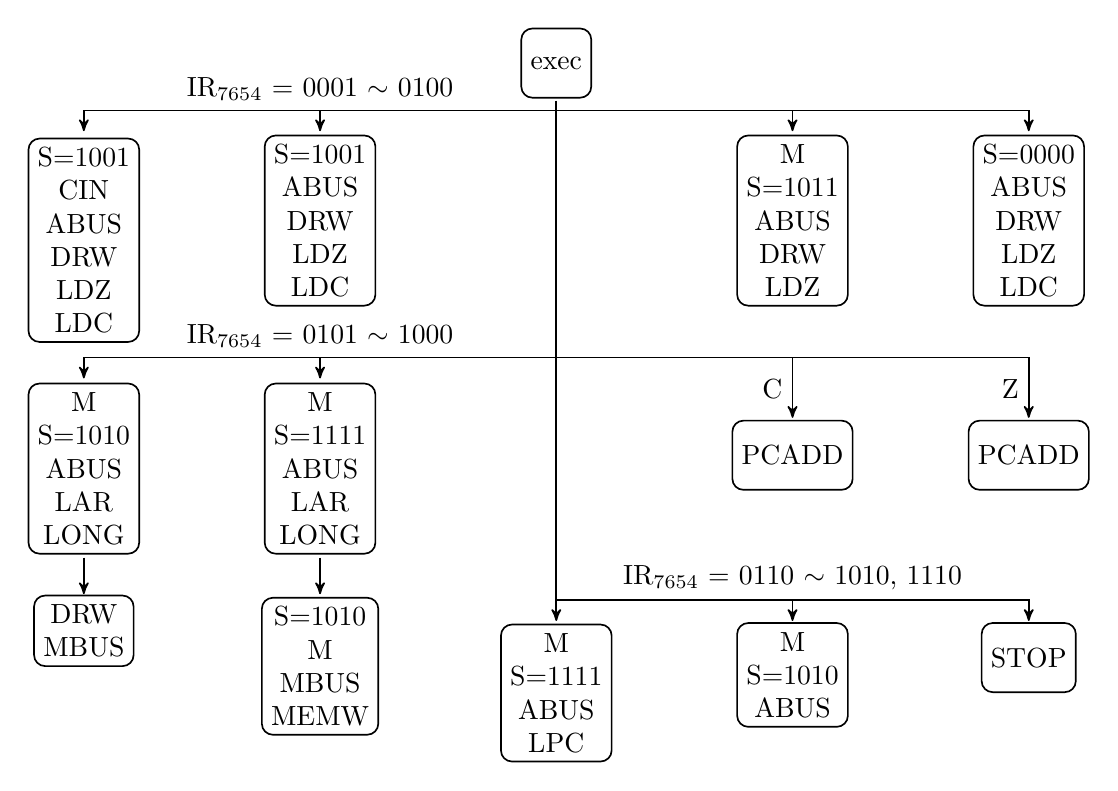
\begin{tikzpicture}[->,>=stealth',shorten >=1pt,auto,node distance=2.8cm,semithick]
    \tikzstyle{every state}=[shape=rectangle, rounded corners]
	\node [state] (A) at (0, 0) {exec};
	\node [state, align = center] at (-6, -2.25) {S=1001\\ CIN \\ ABUS\\ DRW\\ LDZ\\ LDC};
	
	\node [state, align = center] at (-3, -2) {S=1001 \\ ABUS\\ DRW\\ LDZ\\ LDC};
	
	\node [state, align = center] at (3, -2) {M\\ S=1011 \\ ABUS\\ DRW\\ LDZ};

	\node [state, align = center] at (6, -2) { S=0000 \\ ABUS\\ DRW\\ LDZ\\ LDC};

	\node [state, align = center] at (-6, -5.15) { M\\ S=1010 \\ ABUS\\ LAR\\ LONG};
	
	\node [state, align = center] at (-6, -7.21) {DRW\\ MBUS};

	\node [state, align = center] at (-3, -5.15) { M\\ S=1111 \\ ABUS\\ LAR\\ LONG};

	\node [state, align = center] at (-3, -7.66) {S=1010\\ M\\ MBUS\\ MEMW};
	
	\node [state, align = center] at (3, -4.98) {PCADD};

	\node [state, align = center] at (6, -4.98) {PCADD};
	
	\node [state, align = center] at (0, -8) {M\\S=1111\\ ABUS\\ LPC};

	\node [state, align = center] at (3, -7.77) {M\\S=1010\\ ABUS};
	
	\node [state, align = center] at (6, -7.55) {STOP};
	
	\draw [->] (0, -0.48) -- (0, -0.6) -- (-6, -0.6) -- (-6, -0.9);
	\draw [->] (-3, -0.6) -- (-3, -0.9);
	\draw [->] (0, -0.48) -- (0, -0.6) -- (6, -0.6) -- (6, -0.9);
	\draw [->] (3, -0.6) -- (3, -0.9);

	\draw [->] (0, -0.6) -- (0, -3.74) -- (-6, -3.74) -- (-6, -4.04);
	\draw [->] (-3, -3.74) -- (-3, -4.04);
	\draw [->] (0, -3.74) -- (6, -3.74) -- node [left]{Z} (6, -4.54);
	\draw [->] (3, -3.74) -- node [left]{C} (3, -4.54);

	\draw [->] (0, -3.74) -- (0, -6.82) -- (0, -7.12);
	\draw [->] (0, -6.82) -- (6, -6.82) -- (6, -7.12);
	\draw [->] (3, -6.82) -- (3, -7.12);
	\draw [->] (-6, -6.28) -- (-6, -6.78);
	\draw [->] (-3, -6.28) -- (-3, -6.78);
	
	\node [above] at (-3, -0.6) {$\text{IR}_{7654}$ = 0001 $\sim$ 0100};
	\node [above] at (-3, -3.74) {$\text{IR}_{7654}$ = 0101 $\sim$ 1000};
	\node [above] at (3, -6.82) {$\text{IR}_{7654}$ = 0110 $\sim$ 1010, 1110};
	\end{tikzpicture}
\end{figure}\\
\indent 上图显示了从左到右,从上到下依次为ADD, SUB, AND, INC, LD, ST, JC, JZ, JMP, OUT, STP的所有指令, 为了画图方便, 没有列入的指令为DEC(0000), SSP(1011), PUSHS(1100), MOV(1101), POPS(1111).\\
\indent 我们将NOP指令(空指令)改为了DEC指令,这不影响程序的正确性,因为JMP指令可以代NOP完成地址跳转.\\
\indent 需要注意的是, 如果某条指令包含SHORT, 那么它是一个单拍指令, 如果某条指令包含LONG,那么它的下一拍还属于该指令, 计三拍.\\
\indent 关于指令的具体说明,参考流水硬连线的各指令说明,因为这两者除了流水的特征没有其他区别.
\subsubsection{翻译成硬连线信号}
这一步比较简单,按照$SWC, SWB, SWA, IR_{7654}$将状态编号,依此对信号进行组合.\\
\noindent SBUS $\leftarrow$
\begin{enumerate}[\indent\indent]
	\item $(\text{W1} + \text{W2}) \cdot \text{SWC} \cdot \overline{\text{SWB}} \cdot \overline{\text{SWA}}$+
	\item $\text{W1} \cdot \overline{\text{SWC}} \cdot \text{SWB} \cdot \overline{\text{SWA}} \cdot \overline {\text{ST0}}$+
	\item $\text{W1} \cdot \overline{\text{SWC}} \cdot\overline{\text{SWB}}\cdot  \text{SWA}$+
​	\item $\text{W1} \cdot \overline{\text{SWC}} \cdot\overline{\text{SWB}}\cdot \overline{\text{SWA}}\cdot \overline{\text{ST0}} $
\end{enumerate}
MBUS $\leftarrow$
\begin{enumerate}[\indent\indent]
	\item $\text{W1} \cdot \overline{\text{SWC}} \cdot \text{SWB} \cdot \overline{\text{SWA}} \cdot \text{ST0}$+
	\item $\text{W3} \cdot \overline{\text{IR7}} \cdot \text{IR6} \cdot \overline{\text{IR5}} \cdot \text{IR4} \cdot \overline{\text{SWC}} \cdot\overline{\text{SWB}}\cdot \overline{\text{SWA}}$
\end{enumerate}
ABUS $\leftarrow$
\begin{enumerate}[\indent\indent]
	\item $\overline{\text{SWC}} \cdot\overline{\text{SWB}}\cdot \overline{\text{SWA}} \cdot \overline{\text{IR7}} \cdot \overline{\text{IR6}} \cdot \overline{\text{IR5}} \cdot \text{IR4} \cdot \text{W2}$+

​	\item $\overline{\text{SWC}} \cdot\overline{\text{SWB}}\cdot \overline{\text{SWA}} \cdot \overline{\text{IR7}} \cdot \overline{\text{IR6}} \cdot \overline{\text{IR5}} \cdot \overline{\text{IR4} }\cdot \text{W2}$+

​	\item $\overline{\text{SWC}} \cdot\overline{\text{SWB}}\cdot \overline{\text{SWA}} \cdot \overline{\text{IR7}} \cdot \overline{\text{IR6}} \cdot \text{IR5} \cdot \overline{\text{IR4}} \cdot \text{W2}$+
​	\item $\overline{\text{SWC}} \cdot\overline{\text{SWB}}\cdot \overline{\text{SWA}} \cdot \overline{\text{IR7}} \cdot \overline{\text{IR6}} \cdot \text{IR5} \cdot \text{IR4} \cdot \text{W2}$+
​	\item $\overline{\text{SWC}} \cdot\overline{\text{SWB}}\cdot \overline{\text{SWA}} \cdot \overline{\text{IR7}} \cdot \text{IR6} \cdot \overline{\text{IR5}} \cdot \overline{\text{IR4}} \cdot \text{W2}$+
​	\item $\overline{\text{SWC}} \cdot\overline{\text{SWB}}\cdot \overline{\text{SWA}} \cdot \overline{\text{IR7}} \cdot \text{IR6} \cdot \overline{\text{IR5}} \cdot \text{IR4} \cdot \text{W2}$+
​	\item $\overline{\text{SWC}} \cdot\overline{\text{SWB}}\cdot \overline{\text{SWA}} \cdot \overline{\text{IR7}} \cdot \text{IR6} \cdot \text{IR5} \cdot \overline{\text{IR4}} \cdot (\text{W2} + \text{W3})$+
​	\item $\overline{\text{SWC}} \cdot\overline{\text{SWB}}\cdot \overline{\text{SWA}} \cdot \text{IR7} \cdot \overline{\text{IR6}} \cdot \overline{\text{IR5}} \cdot \text{IR4} \cdot \text{W2}$+
​	\item $\overline{\text{SWC}} \cdot\overline{\text{SWB}}\cdot \overline{\text{SWA}} \cdot \text{IR7} \cdot \overline{\text{IR6}} \cdot \text{IR5} \cdot \overline{\text{IR4}} \cdot \text{W2}$
\end{enumerate}
LAR $\leftarrow$
\begin{enumerate}[\indent\indent]
	\item $\text{W1} \cdot \overline{\text{SWC}} \cdot \text{SWB} \cdot \overline{\text{SWA}} \cdot \overline{\text{ST0}}$+
	\item $\text{W1} \cdot \overline{\text{SWC}} \cdot \overline{\text{SWB}} \cdot \text{SWA} \cdot \overline{\text{ST0}}$+
	\item $\overline{\text{SWC}} \cdot\overline{\text{SWB}}\cdot \overline{\text{SWA}}+ \cdot \overline{\text{IR7}} \cdot \text{IR6} \cdot \overline{\text{IR5}} \cdot \text{IR4} \cdot \text{W2}$+
	\item $\overline{\text{SWC}} \cdot\overline{\text{SWB}}\cdot \overline{\text{SWA}}+ \cdot \overline{\text{IR7}} \cdot \text{IR6} \cdot \text{IR5} \cdot \overline{\text{IR4}} \cdot \text{W2}$
\end{enumerate}
SST0 $\leftarrow$
\begin{enumerate}[\indent\indent]
	\item $\text{W1} \cdot \overline{\text{SWC}} \cdot \text{SWB} \cdot \overline{\text{SWA}} \cdot \overline{\text{ST0}}$+
	\item $\text{W2} \cdot \text{SWC} \cdot \overline{\text{SWB}} \cdot \overline{\text{SWA}} \cdot \overline{\text{ST0}}$+
	\item $\text{W1} \cdot \overline{\text{SWC}} \cdot \overline{\text{SWB}} \cdot \text{SWA} \cdot \overline{\text{ST0}}$+
	\item $\text{W1} \cdot \overline{\text{SWC}} \cdot \overline{\text{SWB}} \cdot \overline{\text{SWA}} \cdot \overline{\text{ST0}}$
\end{enumerate}
SHORT $\leftarrow$
\begin{enumerate}[\indent\indent]
	\item $\text{W1} \cdot \overline{\text{SWC}} \cdot \text{SWB} \cdot \overline{\text{SWA}}$+
	\item $\text{W1} \cdot \overline{\text{SWC}} \cdot \overline{\text{SWB}} \cdot \text{SWA}$+
	\item $\text{W1} \cdot \overline{\text{SWC}} \cdot \overline{\text{SWB}} \cdot \overline{\text{SWA}} \cdot \overline{ST0}$
\end{enumerate}
ARINC $\leftarrow$
\begin{enumerate}[\indent\indent]
	\item $\text{W1} \cdot \overline{\text{SWC}} \cdot \text{SWB} \cdot \overline{\text{SWA}} \cdot \text{ST0}$+
	\item $\text{W1} \cdot \overline{\text{SWC}} \cdot \overline{\text{SWB}} \cdot \text{SWA} \cdot \text{ST0}$
\end{enumerate}
MEMW $\leftarrow$
\begin{enumerate}[\indent\indent]
	\item $\text{W1} \cdot \overline{\text{SWC}} \cdot \overline{\text{SWB}} \cdot \text{SWA} \cdot \text{ST0}$+
	\item $\overline{\text{SWC}} \cdot\overline{\text{SWB}}\cdot \overline{\text{SWA}} \cdot \overline{\text{IR7}} \cdot \text{IR6} \cdot \text{IR5} \cdot \overline{\text{IR4}} \cdot \text{W3}$
\end{enumerate}
LIR $\leftarrow$
\begin{enumerate}[\indent\indent]
	\item $\overline{\text{SWC}} \cdot\overline{\text{SWB}}\cdot \overline{\text{SWA}} \cdot \text{ST0} \cdot \text{W1}$
\end{enumerate}
CIN $\leftarrow$
\begin{enumerate}[\indent\indent]
	\item $\overline{\text{SWC}} \cdot\overline{\text{SWB}}\cdot \overline{\text{SWA}} \cdot \overline{\text{IR7}} \cdot \overline{\text{IR6}} \cdot \overline{\text{IR5}} \cdot \overline{\text{IR4} }\cdot \text{W2}$+
	\item $\overline{\text{SWC}} \cdot\overline{\text{SWB}}\cdot \overline{\text{SWA}} \cdot \overline{\text{IR7}} \cdot \overline{\text{IR6}} \cdot \overline{\text{IR5}} \cdot \overline{\text{IR4}} \cdot \text{W2}$
\end{enumerate}
M $\leftarrow$
\begin{enumerate}[\indent\indent]
	\item $\overline{\text{SWC}} \cdot\overline{\text{SWB}}\cdot \overline{\text{SWA}} \cdot \overline{\text{IR7}} \cdot \overline{\text{IR6}} \cdot \text{IR5} \cdot \text{IR4} \cdot \text{W2}$+
	\item $\overline{\text{SWC}} \cdot\overline{\text{SWB}}\cdot \overline{\text{SWA}} \cdot \overline{\text{IR7}} \cdot \text{IR6} \cdot \overline{\text{IR5}} \cdot \text{IR4} \cdot \text{W2}$+
	\item $\overline{\text{SWC}} \cdot\overline{\text{SWB}}\cdot \overline{\text{SWA}} \cdot \overline{\text{IR7}} \cdot \text{IR6} \cdot \text{IR5} \cdot \overline{\text{IR4}} \cdot (\text{W2} + \text{W3})$+
	\item $\overline{\text{SWC}} \cdot\overline{\text{SWB}}\cdot \overline{\text{SWA}} \cdot \text{IR7} \cdot \overline{\text{IR6}} \cdot \overline{\text{IR5}} \cdot \text{IR4} \cdot \text{W2}$+
	\item $\overline{\text{SWC}} \cdot\overline{\text{SWB}}\cdot \overline{\text{SWA}} \cdot \text{IR7} \cdot \overline{\text{IR6}} \cdot \text{IR5} \cdot \overline{\text{IR4}} \cdot \text{W2}$
\end{enumerate}
SEL0$\leftarrow$
\begin{enumerate}[\indent\indent]
	\item$\text{SWC}\cdot\overline{\text{SWB}}\cdot\overline{\text{SWA}}\cdot\text{W1}$
\end{enumerate}
SEL1$\leftarrow$
\begin{enumerate}[\indent\indent]
	\item$\text{SWC}\cdot\overline{\text{SWB}}\cdot\overline{\text{SWA}}\cdot\text{W2}\cdot\text{ST0}$
	\item$\text{SWC}\cdot\overline{\text{SWB}}\cdot\overline{\text{SWA}}\cdot\text{W1}\cdot\overline{\text{ST0}}$
\end{enumerate}
SEL2$\leftarrow$
\begin{enumerate}[\indent\indent]
	\item$\text{SWC}\cdot\overline{\text{SWB}}\cdot\overline{\text{SWA}}\cdot\text{W2}$
\end{enumerate}
SEL3$\leftarrow$
\begin{enumerate}[\indent\indent]
	\item$\text{SWC}\cdot\overline{\text{SWB}}\cdot\overline{\text{SWA}}\cdot\text{W1}\cdot\text{ST0}$+
	\item$\text{SWC}\cdot\overline{\text{SWB}}\cdot\overline{\text{SWA}}\cdot\text{W2}\cdot\overline{\text{ST0}}$
\end{enumerate}		
STOP$\leftarrow$
\begin{enumerate}[\indent\indent]
	\item$\text{SWA}+\text{SWB}+\text{SWC}$+
	\item$\overline{\text{SWC}}\cdot\overline{\text{SWB}}\cdot\overline{\text{SWA}}\cdot {\text{IR7}} \cdot {\text{IR6}}\cdot {\text{IR5}}\cdot \overline{\text{IR4}} \cdot \text{ST0}\cdot \text{W2}$
\end{enumerate}
SELCTL$\leftarrow$
\begin{enumerate}[\indent\indent]
	\item$\text{SWA}+\text{SWB}+\text{SWC}$
\end{enumerate}
DRW$\leftarrow$
\begin{enumerate}[\indent\indent]
	\item$\text{SWC}\cdot\overline{\text{SWB}}\cdot\overline{\text{SWA}}$+
	\item $\overline{\text{SWC}} \cdot\overline{\text{SWB}}\cdot \overline{\text{SWA}} \cdot \overline{\text{IR7}} \cdot \overline{\text{IR6}} \cdot \overline{\text{IR5}} \cdot \overline{\text{IR4} }\cdot \text{W2}$+	
	\item$\overline{\text{SWC}}\cdot\overline{\text{SWB}}\cdot\overline{\text{SWA}}\cdot\text{ST0}\cdot\overline{\text{IR7}}\cdot\overline{\text{IR6}}\cdot\overline{\text{IR5}}\cdot\text{IR4}\cdot\text{W2}$+	
	\item$\overline{\text{SWC}}\cdot\overline{\text{SWB}}\cdot\overline{\text{SWA}}\cdot\text{ST0}\cdot\overline{\text{IR7}}\cdot\overline{\text{IR6}}\cdot{\text{IR5}}\cdot\overline{\text{IR4}}\cdot\text{W2}$+
	\item$\overline{\text{SWC}}\cdot\overline{\text{SWB}}\cdot\overline{\text{SWA}}\cdot\text{ST0}\cdot\overline{\text{IR7}}\cdot\overline{\text{IR6}}\cdot\text{IR5}\cdot\text{IR4}\cdot\text{W2}$+
	\item$\overline{\text{SWC}}\cdot\overline{\text{SWB}}\cdot\overline{\text{SWA}}\cdot\text{ST0}\cdot\overline{\text{IR7}}\cdot{\text{IR6}}\cdot\overline{\text{IR5}}\cdot\overline{\text{IR4}}\cdot\text{W2}$+
	\item$\overline{\text{SWC}}\cdot\overline{\text{SWB}}\cdot\overline{\text{SWA}}\cdot\text{ST0}\cdot\overline{\text{IR7}}\cdot{\text{IR6}}\cdot\overline{\text{IR5}}\cdot{\text{IR4}}\cdot\text{W3}$
\end{enumerate}
PCADD$\leftarrow$
\begin{enumerate}[\indent\indent]
	\item$\overline{\text{SWC}}\cdot\overline{\text{SWB}}\cdot\overline{\text{SWA}}\cdot\text{ST0}\cdot\overline{\text{IR7}}\cdot{\text{IR6}}\cdot{\text{IR5}}\cdot{\text{IR4}}\cdot\text{C}\cdot\text{W2}$+
	\item$\overline{\text{SWC}}\cdot\overline{\text{SWB}}\cdot\overline{\text{SWA}}\cdot\text{ST0}\cdot{\text{IR7}}\cdot\overline{\text{IR6}}\cdot\overline{\text{IR5}}\cdot\overline{\text{IR4}}\cdot\text{Z}\cdot\text{W2}$
\end{enumerate}
PCINC$\leftarrow$
\begin{enumerate}[\indent\indent]
	\item$\overline{\text{SWC}}\cdot\overline{\text{SWB}}\cdot\overline{\text{SWA}}\cdot\text{ST0}\cdot\text{W1}$
\end{enumerate}
LPC$\leftarrow$
\begin{enumerate}[\indent\indent]
	\item$\overline{\text{SWC}}\cdot\overline{\text{SWB}}\cdot\overline{\text{SWA}}\cdot\overline{\text{ST0}}\cdot\text{W2}$
\end{enumerate}
LONG$\leftarrow$
\begin{enumerate}[\indent\indent]
	\item$\overline{\text{SWC}}\cdot\overline{\text{SWB}}\cdot\overline{\text{SWA}}\cdot\text{W2}\cdot\overline{\text{IR7}}\cdot{\text{IR6}}\cdot\overline{\text{IR5}}\cdot{\text{IR4}}$+
	\item$\overline{\text{SWC}}\cdot\overline{\text{SWB}}\cdot\overline{\text{SWA}}\cdot\text{W2}\cdot\overline{\text{IR7}}\cdot{\text{IR6}}\cdot{\text{IR5}}\cdot\overline{\text{IR4}}$
\end{enumerate}

LDC$\leftarrow$
\begin{enumerate}[\indent\indent]
	\item$\overline{\text{SWC}}\cdot\overline{\text{SWB}}\cdot\overline{\text{SWA}}\cdot\text{ST0}\cdot\overline{\text{IR7}}\cdot\overline{\text{IR6}}\cdot\overline{\text{IR5}}\cdot\text{IR4}\cdot\text{W2}$+
	\item $\overline{\text{SWC}} \cdot\overline{\text{SWB}}\cdot \overline{\text{SWA}} \cdot \overline{\text{IR7}} \cdot \overline{\text{IR6}} \cdot \overline{\text{IR5}} \cdot \overline{\text{IR4} }\cdot \text{W2}$+\item$\overline{\text{SWC}}\cdot\overline{\text{SWB}}\cdot\overline{\text{SWA}}\cdot\text{ST0}\cdot\overline{\text{IR7}}\cdot\overline{\text{IR6}}\cdot{\text{IR5}}\cdot\overline{\text{IR4}}\cdot\text{W2}$+
	\item$\overline{\text{SWC}}\cdot\overline{\text{SWB}}\cdot\overline{\text{SWA}}\cdot\text{ST0}\cdot\overline{\text{IR7}}\cdot\overline{\text{IR6}}\cdot\text{IR5}\cdot\text{IR4}\cdot\text{W2}$+
	\item$\overline{\text{SWC}}\cdot\overline{\text{SWB}}\cdot\overline{\text{SWA}}\cdot\text{ST0}\cdot\overline{\text{IR7}}\cdot{\text{IR6}}\cdot\overline{\text{IR5}}\cdot\overline{\text{IR4}}\cdot\text{W2}$
\end{enumerate}
LDZ$\leftarrow$
\begin{enumerate}[\indent\indent]
	\item$\overline{\text{SWC}}\cdot\overline{\text{SWB}}\cdot\overline{\text{SWA}}\cdot\text{ST0}\cdot\overline{\text{IR7}}\cdot\overline{\text{IR6}}\cdot\overline{\text{IR5}}\cdot\text{IR4}\cdot\text{W2}$+
	\item $\overline{\text{SWC}} \cdot\overline{\text{SWB}}\cdot \overline{\text{SWA}} \cdot \overline{\text{IR7}} \cdot \overline{\text{IR6}} \cdot \overline{\text{IR5}} \cdot \overline{\text{IR4} }\cdot \text{W2}$+\item$\overline{\text{SWC}}\cdot\overline{\text{SWB}}\cdot\overline{\text{SWA}}\cdot\text{ST0}\cdot\overline{\text{IR7}}\cdot\overline{\text{IR6}}\cdot{\text{IR5}}\cdot\overline{\text{IR4}}\cdot\text{W2}$+
	\item$\overline{\text{SWC}}\cdot\overline{\text{SWB}}\cdot\overline{\text{SWA}}\cdot\text{ST0}\cdot\overline{\text{IR7}}\cdot\overline{\text{IR6}}\cdot\text{IR5}\cdot\text{IR4}\cdot\text{W2}$+
	\item$\overline{\text{SWC}}\cdot\overline{\text{SWB}}\cdot\overline{\text{SWA}}\cdot\text{ST0}\cdot\overline{\text{IR7}}\cdot{\text{IR6}}\cdot\overline{\text{IR5}}\cdot\overline{\text{IR4}}\cdot\text{W2}$
\end{enumerate}

\subsubsection{翻译成多分支程序}
观察硬连线信号,事实上如果写成VHDL语句,我们可以将SWCBA信号合并.然后再在$\overline{\text{SWC}}\cdot \overline{\text{SWB}}\cdot \overline{\text{SWA}}$分支上将$\text{IR}_{7654}$合并.用两个大switch语句完成逻辑分类.
{\firacode
\begin{lstlisting}[language={VHDL}]
library IEEE;
use IEEE.std_logic_1164.all;
use IEEE.std_logic_unsigned.all;
entity CPU is
	port (
		CLR,C,Z,T3,W1,W2,W3: in std_logic;
		IRH:in std_logic_vector(3 downto 0);
		SWCBA:in std_logic_vector(2 downto 0);
		SELCTL,ABUS,M,SEL1,SEL0,SEL2,SEL3,DRW,SBUS,LIR,MBUS,MEMW,LAR,ARINC,LPC,
		PCINC,PCADD,CIN,LONG,SHORT,STOP,LDC,LDZ: out std_logic;
		S:out std_logic_vector(3 downto 0);
		CP1,CP2,CP3:out std_logic;	
		QD:in std_logic	
	);
end CPU;

architecture arc of CPU is
signal ST0,ST0_1,ST0_2,STOP_1,STOP_2: std_logic;
begin
	CP1 <= '1';
	CP2 <= '1';
	CP3 <= QD;
	
	with SWCBA select
		STOP <= '0'                when "000",
		STOP_1 or STOP_2           when others;
	ST0 <= ST0_1;

	process (CLR, T3)
	begin
		-- 任何时候按下CLR, 都会返回
		if (CLR = '0') then
			ST0_1	<= '0';
			STOP_1	<= '1';
		-- 如果到节拍电位T3下降沿,ST0_1 |= ST0_2
		elsif (T3'event and T3 = '0') then
			if (ST0_2 = '1') then
				ST0_1 <= '1';
			end if;
		end if;
	end process;
	
	process (SWCBA, IRH, W1, W2, W3, ST0, C, Z)
	begin	
		-- 初始化 和 状态参数
		SHORT <= '0';
		LONG <= '0';
		-- 设置STOP
		STOP_2 <= '1';
		-- 设置ST0标志
		ST0_2 <= '0';
		-- ALU
		ABUS <= '0';
		M <= '0';
		CIN <= '0';
		S <= "0000";
		ARINC <= '0';
		-- 保存Z标志
		LDZ <= '0';
		-- 保存C标志
		LDC <= '0';		
		SBUS <= '0';
		MBUS <= '0';
		-- 控制台操作标志
		SELCTL <= '0';
		-- RD1~RD0
		SEL3 <= '0';
		SEL2 <= '0';
		-- RS1~RS0
		SEL1 <= '0';
		SEL0 <= '0';
		-- 送指令寄存器标志
		LIR <= '0';
		-- 送地址寄存器标志
		LAR <= '0';
		-- 送程序计数器标志
		LPC <= '0';
		-- (~R)/W
		MEMW <= '0';
		DRW <= '0';
		-- 程序计数器自增标志
		PCINC <= '0';		
		-- 程序计数器增量标志
		PCADD <= '0';
		case SWCBA is
			when "000" =>  --执行程序
				case ST0 is
					when '0' =>
						-- load pc
						LPC <= W1;
						SBUS <= W1;
						ST0_2 <= W1;
						SHORT <= W1;
						STOP_2 <= '0';
					when '1' =>
						if(W1='1')then
							LIR<=W1;
							PCINC<=W1;
						else                        
					case IRH is 
						when "0001" =>  --ADD 														
							-- ABUS = W2
							ABUS <= W2;
							CIN <= W2;
							-- 选择加法
							-- 选择算术运算, M已经被初始化为0
							S <= "1001";
							-- 加法操作
							DRW <= W2;
							LDZ <= W2;
							LDC <= W2;
						when "0010" =>  -- SUB													
							-- 选择算术运算, 选择减法
							-- M已经被初始化为0
							S <= "0110";
							-- 减法操作
							ABUS <= W2;
							DRW <= W2;
							LDZ <= W2;
							LDC <= W2;
						when "0011" =>  -- AND								
							-- 选择逻辑运算, 与运算
							M <= W2;
							S <= "1011";
							ABUS <= W2;
							DRW <= W2;
							LDZ <= W2;
						when "0100" => -- INC								
							-- 选择算术运算, 与运算
							-- M已经被初始化为0
							S <= "0000";
							ABUS <= W2;
							DRW <= W2;
							LDZ <= W2;
							LDC <= W2;
						when "0101" =>  -- LD
							-- 选择算术运算,传送B(保留原值)
							M <= W2;
							S <= "1010";
							ABUS <= W2;
							LONG<=W2;
							LAR <= W2;
							MBUS <= W3;
							DRW <= W3;
						when "0110" =>  -- ST
							LONG<=W2;
							-- 设定...
							M <= W2 or W3;
							if(W2='1')then
								S<="1111";
							else
								S<="1010";
							end if;
							ABUS <= W2 or W3;
							LAR <= W2;
							MEMW <= W3;							
						when "0111" =>  -- JC
							PCADD <= C and W2;
						when "1000" =>  -- JZ
							PCADD <= Z and W2;
						when "1001" =>  -- JMP
							-- 设定算术运算
							M <= W2;
							S <= "1111";
							ABUS <= W2;
							LPC <= W2;
						when "1010" =>  -- OUT
							-- 设定算术运算
							M <= W2;
							S <= "1010";
							ABUS <= W2;
						when "1011" =>  -- SSP  
							SEL3<='1';
							LONG<=W2;
							M <= W2 or W3;
							if (W2 = '1') then
								S <= "1000";
							elsif (W3 = '1') then
								S <= "1010";
							end if;
							ABUS <= W2 or W3;
							LAR <= W2;
							MEMW <= W3;
						when "1100" =>  -- PUSH
							--PUSH无法自减
							M <= W2 or W3;
							if (W2 = '1') then
								S <= "1111";
							elsif (W3 = '1') then
								S <= "1010";
							end if;
							ABUS <=W2 or W3;
							LAR <= W2;
							MEMW <= W3;
							LONG <= W2;
						when "1101" =>  -- MOV B->A								
							-- 选择逻辑运算, MOV 运算
							M <= W2;
							S <= "1010";
							ABUS <= W2;
							DRW <= W2;
							LDZ <= W2;
						when "1110" =>  -- STP
							STOP_2 <= W2;								
						when "1111" =>  -- LSP
							LONG<=W2;
							M <= W2;
							S <= "1000";
							ABUS <= W2;
							LAR <= W2;
							MBUS <= W3;
							DRW <= W3;		
						when others =>  -- 公操作
					end case;
						end if;
					when others =>
							-- 不可能到这吧?
				end case;
			when "001" =>
			--	SEL0<=ST0;
				-- SBUS = (ST0=0 or ST0=1) and W1 
				SBUS <= W1;
				-- STOP = (ST0=0 or ST0=1) and W1
				STOP_2 <= W1;
				-- SHORT = (ST0=0 or ST0=1) and W1
				SHORT <= W1;
				-- SELCTL = (ST0=0 or ST0=1) and W1
				SELCTL <= W1;
				-- LAR = (ST0=0) and W1
				LAR <= W1 and (not ST0);
				-- LAR = (ST0=1) and W1
				ARINC <= W1 and ST0;
				-- MEMW = (ST0=1) and W1
				MEMW <= W1 and ST0;
				ST0_2 <= W1;
			when "010" =>
				-- SHORT = (ST0=0 or ST0=1) and W1
				SHORT<=W1;
				-- SELCTL = (ST0=0 or ST0=1) and W1
				SELCTL <= W1;
				-- STOP = (ST0=0 or ST0=1) and W1
				STOP_2<=W1;
				-- SBUS = (ST0=0) and W1
				SBUS<=W1 and (not ST0);
				-- LAR = (ST0=0) and W1
				LAR<=W1 and (not ST0);
				-- MBUS = (ST0=1) and W1
				MBUS<=W1 and ST0;
				-- ARINC = (ST0=1) and W1
				ARINC<=W1 and ST0;
				ST0_2<=W1;
			when "011" =>
				-- SELCTL = W1 or W2
				SELCTL <= '1';
				-- STOP = W1 or W2
				STOP_2 <= W1 or W2;
				-- SEL0 = W1 or W2
				SEL0<=W1 or W2;
				-- SEL1 = W2
				SEL1<=W2;
				-- SEL2 = 0
				-- SEL3 = W2
				SEL3<=W2;
			when "100" =>
				-- SELCTL = (ST0=0 or ST0=1) and (W1 or W2)
				SELCTL <= '1';
				-- SBUS = (ST0=0 or ST0=1) and (W1 or W2)
				SBUS <= W1 or W2;
				-- STOP = (ST0=0 or ST0=1) and (W1 or W2)
				STOP_2 <= W1 or W2;
				-- DRW = (ST0=0 or ST0=1) and (W1 or W2)
				DRW <= W1 or W2;
				-- SEL0 = (ST0=0 or ST0=1) and W1
				SEL0 <= W1;
				-- SEL1 = ((ST0=0) and W1) or ((ST0=1) and W2)
				SEL1 <= ((not ST0) and W1) or (ST0 and W2);
				-- SEL2 = (ST0=0 or ST0=1) and W2
				SEL2 <= W2;
				-- SEL3 = (ST0=1) and (W1 or W2) 
				SEL3 <= ST0 and (W1 or W2);
				ST0_2 <= W2;
			when others=>
		end case;
	end process;
end arc;
\end{lstlisting}
}
\subsection{流水硬连线控制器}

\subsubsection{指令周期说明}
\begin{figure}[!h]
    \centering
    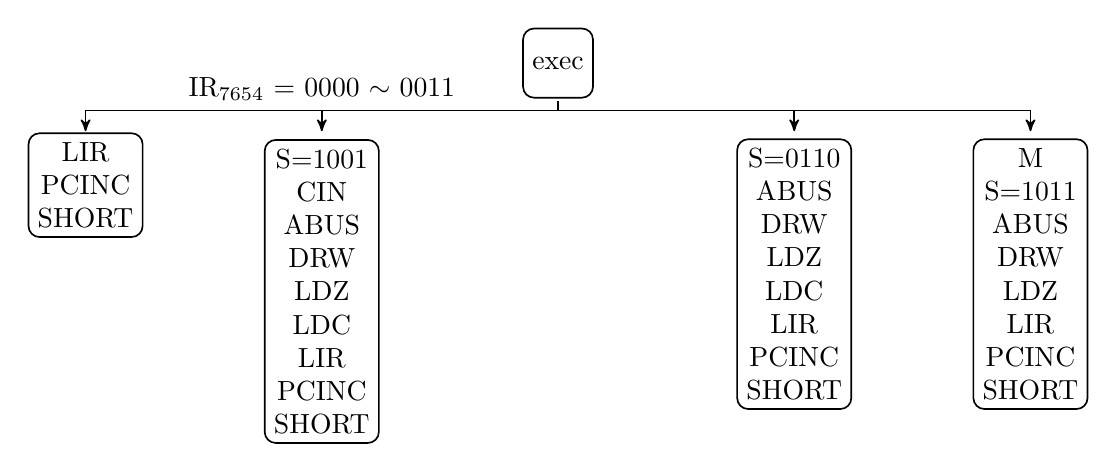
\begin{tikzpicture}[->,>=stealth',shorten >=1pt,auto,node distance=2.8cm,semithick]
    \tikzstyle{every state}=[shape=rectangle, rounded corners, align = center]
	\node [state] (A) at (0, 0) {exec};
	\node [state] at (-6, -1.55) {LIR\\ PCINC\\ SHORT};
	\node [state] at (-3, -2.90) {S=1001\\ CIN \\ ABUS\\ DRW\\ LDZ\\ LDC \\ LIR \\ PCINC \\ SHORT};
	
	\node [state] at (3, -2.68) {S=0110 \\ ABUS\\ DRW\\ LDZ\\ LDC \\ LIR \\ PCINC \\ SHORT};
	
	\node [state] at (6, -2.68) {M\\ S=1011 \\ ABUS\\ DRW\\ LDZ \\ LIR \\ PCINC \\ SHORT};
	\draw [->] (0, -0.48) -- (0, -0.6) -- (-6, -0.6) -- (-6, -0.9);
	\draw [->] (-3, -0.6) -- (-3, -0.9);
	\draw [->] (0, -0.48) -- (0, -0.6) -- (6, -0.6) -- (6, -0.9);
	\draw [->] (3, -0.6) -- (3, -0.9);
	\node [above] at (-3, -0.6) {$\text{IR}_{7654}$ = 0000 $\sim$ 0011};
	\end{tikzpicture}
\end{figure}
上图给出了第一组四个指令的周期.\\
\indent 第一个是NOP空指令,只加载下地址指令,并向控制器发送SHORT信号表明该指令只有一个周期.\\
\indent 第二个是ADD指令.M=0,S=1001表明ALU完成加法运算, CIN=1表明ALU不进1,这时候ALU将A侧寄存器和B侧寄存器作为输入,ABUS将ALU的运算结果$A\text{ plus }B$打入DBUS.DRW将DBUS数据打入A侧寄存器,因此这个指令完成了$A\leftarrow A\text{ plus }B$.\\
\indent 第三个是SUB指令.M=0,S=0110表明ALU完成减法运算, CIN=0表明ALU进1,这时候ALU将A侧寄存器和B侧寄存器作为输入,ABUS将ALU的运算结果$A\text{ minus }B\text{ minus }1\text{ plus }1$打入DBUS.DRW将DBUS数据打入A侧寄存器,因此这个指令完成了$A\leftarrow A\text{ minus }B$.\\
\indent 第四个是AND指令.M=1,S=1011表明ALU完成且运算,这时候ALU将A侧寄存器和B侧寄存器作为输入,ABUS将ALU的运算结果$AB$打入DBUS.DRW将DBUS数据打入A侧寄存器,因此这个指令完成了$A\leftarrow AB$.
\newpage
\begin{figure}[!h]
    \centering
    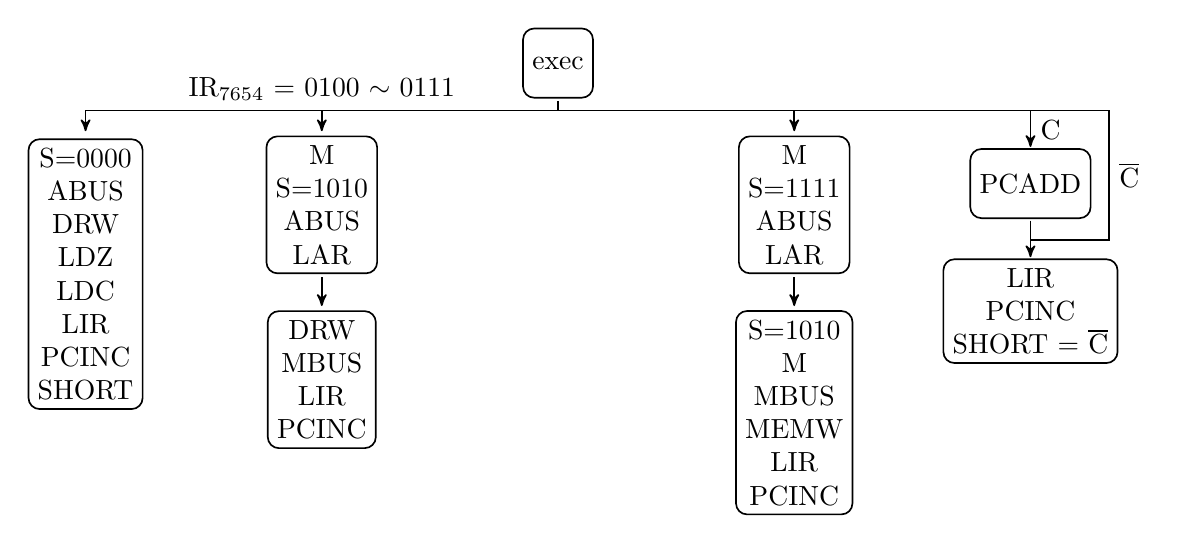
\begin{tikzpicture}[->,>=stealth',shorten >=1pt,auto,node distance=2.8cm,semithick]
    \tikzstyle{every state}=[shape=rectangle, rounded corners, align = center]
	\node [state] (A) at (0, -4.85) {exec};
	\node [state] at (-6, -7.53) { S=0000 \\ ABUS\\ DRW\\ LDZ\\ LDC \\ LIR \\ PCINC \\ SHORT};

	\node [state] at (-3, -6.65) { M\\ S=1010 \\ ABUS\\ LAR};
	
	\node [state] at (-3, -8.87) {DRW\\ MBUS\\ LIR\\ PCINC};

	\node [state] at (3, -6.65) { M\\ S=1111 \\ ABUS\\ LAR};

	\node [state] at (3, -9.29) {S=1010\\ M\\ MBUS\\ MEMW\\ LIR\\ PCINC};
	
	\node [state] at (6, -6.38) {PCADD};
	
	\node [state] at (6, -8) {LIR\\ PCINC\\ SHORT = $\overline{\text{C}}$};
	
	\draw [->] (0, -5.33) -- (0, -5.45) -- (-6, -5.45) -- (-6, -5.75);
	\draw [->] (-3, -5.45) -- (-3, -5.75);
	\draw [->] (0, -5.45) -- (6, -5.45) -- node[right]{C} (6, -5.95);
	\draw [-] (6, -5.45) -- (7, -5.45) --node[right]{$\overline{\text{C}}$} (7, -7.1) -- (5.97, -7.1);
	\draw [->] (3, -5.45) -- (3, -5.75);
	
	\draw [->] (-3, -7.57) -- (-3, -7.97);
	\draw [->] (3, -7.57) -- (3, -7.97);
	\draw [->] (6, -6.85) -- (6, -7.35);
	\node [above] at (-3, -5.45) {$\text{IR}_{7654}$ = 0100 $\sim$ 0111};
	\end{tikzpicture}
\end{figure}
上图给出了第二组四个指令的周期.\\
\indent 第五个指令是INC指令.M=0, S=0000表明ALU完成自输出运算,CIN=0表明ALU进1,这时候ALU将A侧寄存器作为输入,ABUS将ALU的运算结果$A$打入DBUS,因此DRW将DBUS数据打入A侧寄存器,因此这个指令完成了$A\leftarrow A \text{ plus } 1$.\\
\indent 第六个指令是LD指令.在指令的第一个周期,M=1,S=1010表明ALU完成自输出.\\
\indent 第七个指令是ST指令.在指令的第一个周期,M=1,S=1111表示把地址送到地址寄存器,第二个周期把数据送上数据总线并且写入存储器.\\
\indent 第八个指令是JC指令.如果当前的C不为1,则直接取下一条的指令结束,如果当前的C为1,会调用PCADD把当前的PC加上偏移的offset,最后还是流水机的取指令共操作.

\begin{figure}[!h]
    \centering
    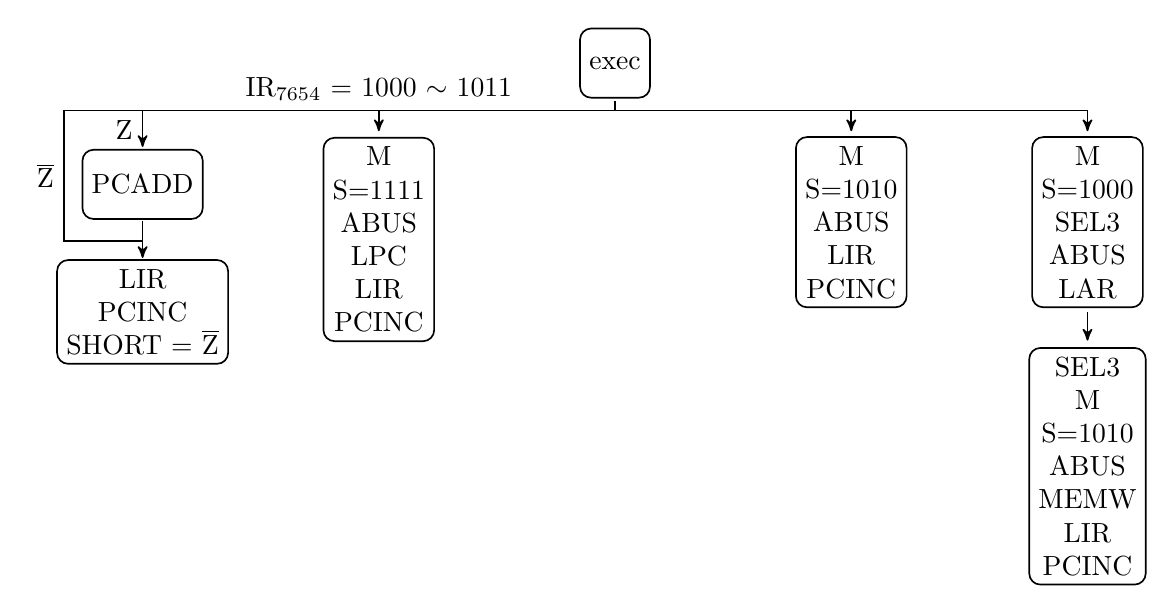
\begin{tikzpicture}[->,>=stealth',shorten >=1pt,auto,node distance=2.8cm,semithick]
    \tikzstyle{every state}=[shape=rectangle, rounded corners, align = center]
	\node [state] (A) at (0, -10.56) {exec};
	
	\node [state] at (-6, -12.1) {PCADD};
	
	\node [state] at (-6, -13.72) {LIR\\ PCINC\\ SHORT = $\overline{\text{Z}}$};
	
	\node [state] at (-3, -12.8) {M\\ S=1111\\ ABUS\\ LPC\\ LIR\\ PCINC};
	\node [state] at (3, -12.58) {M \\ S=1010\\ ABUS\\ LIR\\ PCINC};
	\node [state] at (6, -12.58) { M\\ S=1000\\ SEL3\\ABUS\\ LAR};
	\node [state] at (6, -15.68) {SEL3\\ M\\ S=1010\\ ABUS\\ MEMW\\ LIR\\ PCINC};
	
	\draw [->] (0, -11.04) -- (0, -11.16) -- (-6, -11.16) --node[left]{Z} (-6, -11.66);
	\draw [-] (-6, -11.16) -- (-7, -11.16) --node[left]{$\overline{\text{Z}}$} (-7, -12.82) -- (-5.97, -12.82);
	\draw [->] (-3, -11.16) -- (-3, -11.46);
	\draw [->] (0, -11.16) -- (6, -11.16) -- (6, -11.46);
	\draw [->] (3, -11.16) -- (3, -11.46);

	\draw [->] (-6, -12.57) -- (-6, -13.07);
	\draw [->] (6, -13.72) -- (6, -14.12);
	\node [above] at (-3, -11.16) {$\text{IR}_{7654}$ = 1000 $\sim$ 1011};
	\end{tikzpicture}
\end{figure}
上图给出了第三组四个指令的周期.\\
\indent 第九个指令是JZ指令.如果当前的Z不为1,则直接取下一条的指令结束,如果当前的Z为1,会调用PCADD把当前的PC加上偏移的offset,最后还是流水机的取指令共操作.\\
\indent 第十个指令是JMP指令.第一个周期调用LPC并且打开ABUS开关,把地址送上地址总线,并且写入PC.\\
\indent 第十一个指令是OUT指令.打开ABUS,作用是把数据送上地址总线,方便观察.\\
\indent  第十二个指令是SSP指令.作用是把保存在寄存器中的栈指针SP送回SP在存储器中的位置.这个指令会占用两个周期.由于栈指针SP是隐式给出的,因此需要先算出SP的地址[FF].第一个周期计算$A|(!A)$得到FF,同时打开ABUS把FF送入地址寄存器.第二个周期把数据写入存储器的FF地址.


\begin{figure}[!h]
    \centering
    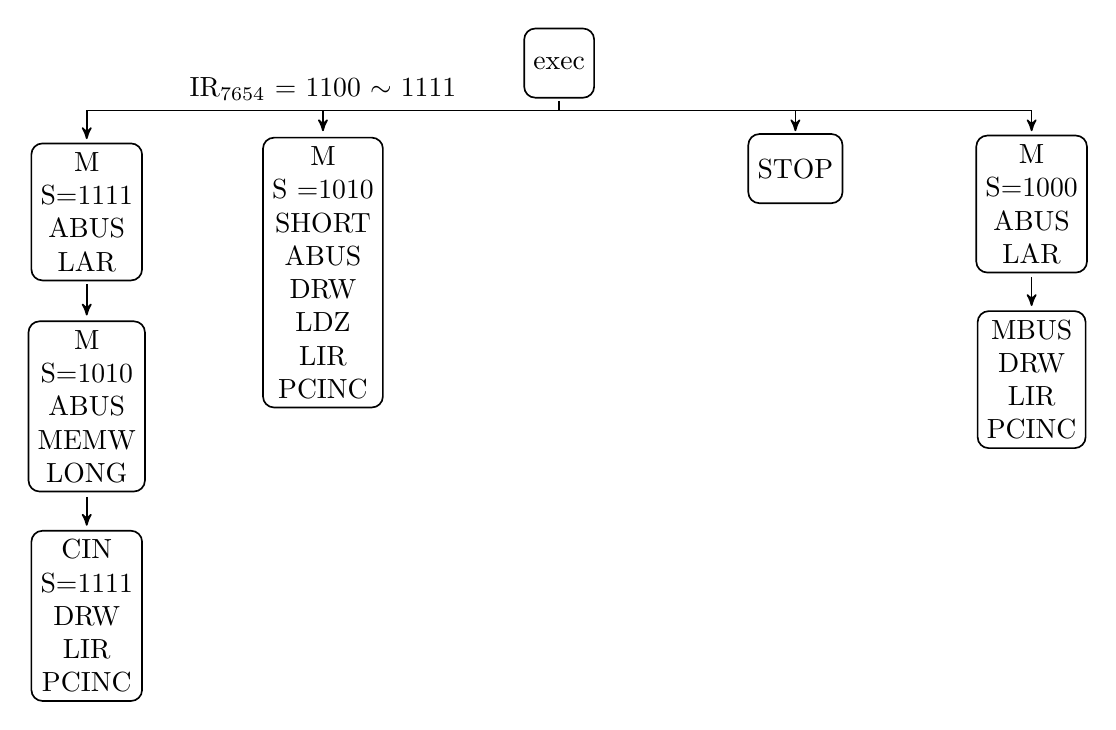
\begin{tikzpicture}[->,>=stealth',shorten >=1pt,auto,node distance=2.8cm,semithick]
    \tikzstyle{every state}=[shape=rectangle, rounded corners, align = center]
	\node [state] (A) at (0, -10.56) {exec};
	\node [state] at (-6, -12.45) {M\\ S=1111\\ ABUS\\ LAR};
	\node [state] at (-6, -14.92)
	{M\\ S=1010\\ ABUS\\ MEMW\\ LONG};
	\node [state] at (-6, -17.58)
	{CIN\\ S=1111\\ DRW\\LIR\\PCINC};
	\node [state] at (-3, -13.22) {M\\ S =1010\\ SHORT\\  ABUS\\ DRW\\ LDZ\\LIR\\ PCINC};
	\node [state] at (3, -11.9) {STOP};
	\node [state] at (6, -12.35) { M\\ S=1000\\ABUS\\ LAR};
	\node [state] at (6, -14.58) {MBUS\\ DRW\\ LIR\\ PCINC};
	\draw [->] (-6, -13.37) -- (-6, -13.8);
	\draw [->] (-6, -16.07) -- (-6, -16.47);
	\draw [->] (0, -11.04) -- (0, -11.16) -- (-6, -11.16) -- (-6, -11.56);
	(-7, -12.82) -- (-5.97, -12.82);
	\draw [->] (-3, -11.16) -- (-3, -11.46);
	\draw [->] (0, -11.16) -- (6, -11.16) -- (6, -11.46);
	\draw [->] (3, -11.16) -- (3, -11.46);

	\draw [->] (6, -13.28) -- (6, -13.68);
	\node [above] at (-3, -11.16) {$\text{IR}_{7654}$ = 1100 $\sim$ 1111};
	\end{tikzpicture}
\end{figure}
上图给出了最后一组四个指令的周期.\\
\indent 第十三个指令是PUSH指令.作用是把数据写入栈顶,并且把栈指针减一.第一周期是把已经读出到寄存器的SP送上地址寄存器,第二周期把数据写入[SP],第三周期把寄存器中的SP减一\\
\indent 第十四个指令是MOV指令.只有一个周期,通过ALU实现A和B计算后输出A,然后把输出写入B.\\
\indent 第十五个指令是STP指令.作用是令STOP信号为1,终止程序.\\
\indent 第十六个指令是LSP指令.作用是把栈指针SP从存储器中读出.第一个周期和STP一样是计算出栈指针的所在位置FF,第二周期从存储器读出SP然后存到指定寄存器.
\subsubsection{翻译成硬连线信号}
SBUS $\leftarrow$
\begin{enumerate}[\indent\indent]
	\item $(\text{W1} + \text{W2}) \cdot \text{SWC} \cdot \overline{\text{SWB}} \cdot \overline{\text{SWA}}$+
	\item $\text{W1} \cdot \overline{\text{SWC}} \cdot \text{SWB} \cdot \overline{\text{SWA}} \cdot \overline {\text{ST0}}$+
	\item $\text{W1} \cdot \overline{\text{SWC}} \cdot\overline{\text{SWB}}\cdot  \text{SWA}$+
​	\item $\text{W1} \cdot \overline{\text{SWC}} \cdot\overline{\text{SWB}}\cdot \overline{\text{SWA}}\cdot \overline{\text{ST0}} $
\end{enumerate}

MBUS $\leftarrow$
\begin{enumerate}[\indent\indent]
	\item $\text{W1} \cdot \overline{\text{SWC}} \cdot \text{SWB} \cdot \overline{\text{SWA}} \cdot \text{ST0}$+
	\item $\text{W2} \cdot \overline{\text{IR7}} \cdot \text{IR6} \cdot \overline{\text{IR5}} \cdot \text{IR4} \cdot \overline{\text{SWC}} \cdot\overline{\text{SWB}}\cdot \overline{\text{SWA}}$
\end{enumerate}

ABUS $\leftarrow$
\begin{enumerate}[\indent\indent]
	\item $\overline{\text{SWC}} \cdot\overline{\text{SWB}}\cdot \overline{\text{SWA}} \cdot \overline{\text{IR7}} \cdot \overline{\text{IR6}} \cdot \overline{\text{IR5}} \cdot \text{IR4} \cdot \text{W1}$+
	\item $\overline{\text{SWC}} \cdot\overline{\text{SWB}}\cdot \overline{\text{SWA}} \cdot \overline{\text{IR7}} \cdot \overline{\text{IR6}} \cdot \text{IR5} \cdot \overline{\text{IR4}} \cdot \text{W1}$+
	\item $\overline{\text{SWC}} \cdot\overline{\text{SWB}}\cdot \overline{\text{SWA}} \cdot \overline{\text{IR7}} \cdot \overline{\text{IR6}} \cdot \text{IR5} \cdot \text{IR4} \cdot \text{W1}$+
	\item $\overline{\text{SWC}} \cdot\overline{\text{SWB}}\cdot \overline{\text{SWA}} \cdot \overline{\text{IR7}} \cdot \text{IR6} \cdot \overline{\text{IR5}} \cdot \overline{\text{IR4}} \cdot \text{W1}$+
	\item $\overline{\text{SWC}} \cdot\overline{\text{SWB}}\cdot \overline{\text{SWA}} \cdot \overline{\text{IR7}} \cdot \text{IR6} \cdot \overline{\text{IR5}} \cdot \text{IR4} \cdot \text{W1}$+
	\item $\overline{\text{SWC}} \cdot\overline{\text{SWB}}\cdot \overline{\text{SWA}} \cdot \overline{\text{IR7}} \cdot \text{IR6} \cdot \text{IR5} \cdot \overline{\text{IR4}} \cdot (\text{W1} + \text{W2})$+
	\item $\overline{\text{SWC}} \cdot\overline{\text{SWB}}\cdot \overline{\text{SWA}} \cdot \text{IR7} \cdot \overline{\text{IR6}} \cdot \overline{\text{IR5}} \cdot \text{IR4} \cdot \text{W1}$+
	\item $\overline{\text{SWC}} \cdot\overline{\text{SWB}}\cdot \overline{\text{SWA}} \cdot \text{IR7} \cdot \overline{\text{IR6}} \cdot \text{IR5} \cdot \overline{\text{IR4}} \cdot \text{W1}$
\end{enumerate}

LAR $\leftarrow$
\begin{enumerate}[\indent\indent]
	\item $\text{W1} \cdot \overline{\text{SWC}} \cdot \text{SWB} \cdot \overline{\text{SWA}} \cdot \overline{\text{ST0}}$+
	\item $\text{W1} \cdot \overline{\text{SWC}} \cdot \overline{\text{SWB}} \cdot \text{SWA} \cdot \overline{\text{ST0}}$+
	\item $\overline{\text{SWC}} \cdot\overline{\text{SWB}}\cdot \overline{\text{SWA}} \cdot \overline{\text{IR7}} \cdot \text{IR6} \cdot \overline{\text{IR5}} \cdot \text{IR4} \cdot \text{W1}$+
	\item $\overline{\text{SWC}} \cdot\overline{\text{SWB}}\cdot \overline{\text{SWA}} \cdot \overline{\text{IR7}} \cdot \text{IR6} \cdot \text{IR5} \cdot \overline{\text{IR4}} \cdot \text{W1}$
\end{enumerate}

SST0 $\leftarrow$
\begin{enumerate}[\indent\indent]
	\item $\text{W1} \cdot \overline{\text{SWC}} \cdot \text{SWB} \cdot \overline{\text{SWA}} \cdot \overline{\text{ST0}}$+
	\item $\text{W2} \cdot \text{SWC} \cdot \overline{\text{SWB}} \cdot \overline{\text{SWA}} \cdot \overline{\text{ST0}}$+
	\item $\text{W1} \cdot \overline{\text{SWC}} \cdot \overline{\text{SWB}} \cdot \text{SWA} \cdot \overline{\text{ST0}}$+
	\item $\text{W1} \cdot \overline{\text{SWC}} \cdot \overline{\text{SWB}} \cdot \overline{\text{SWA}} \cdot \overline{\text{ST0}}$
\end{enumerate}

SHORT $\leftarrow$
\begin{enumerate}[\indent\indent]
	\item $\text{W1} \cdot \overline{\text{SWC}} \cdot \text{SWB} \cdot \overline{\text{SWA}}$
	\item $\text{W1} \cdot \overline{\text{SWC}} \cdot \overline{\text{SWB}} \cdot \text{SWA}$
	\item $\text{W1} \cdot \overline{\text{SWC}} \cdot \overline{\text{SWB}} \cdot \overline{\text{SWA}} \cdot \overline{ST0}$+
	\item $\overline{\text{SWC}} \cdot\overline{\text{SWB}}\cdot \overline{\text{SWA}} \cdot \overline{\text{IR7}} \cdot \overline{\text{IR6}} \cdot \overline{\text{IR5}} \cdot \overline{\text{IR4}} \cdot \text{W1}$+
	\item $\overline{\text{SWC}} \cdot\overline{\text{SWB}}\cdot \overline{\text{SWA}} \cdot \overline{\text{IR7}} \cdot \overline{\text{IR6}} \cdot \overline{\text{IR5}} \cdot \text{IR4} \cdot \text{W1}$+
	\item $\overline{\text{SWC}} \cdot\overline{\text{SWB}}\cdot \overline{\text{SWA}} \cdot \overline{\text{IR7}} \cdot \overline{\text{IR6}} \cdot \text{IR5} \cdot \overline{\text{IR4}} \cdot \text{W1}$+
	\item $\overline{\text{SWC}} \cdot\overline{\text{SWB}}\cdot \overline{\text{SWA}} \cdot \overline{\text{IR7}} \cdot \overline{\text{IR6}} \cdot \text{IR5} \cdot \text{IR4} \cdot \text{W1}$+
	\item $\overline{\text{SWC}} \cdot\overline{\text{SWB}}\cdot \overline{\text{SWA}} \cdot \overline{\text{IR7}} \cdot \text{IR6} \cdot \overline{\text{IR5}} \cdot \overline{\text{IR4}} \cdot \text{W1}$+
	\item $\overline{\text{SWC}} \cdot\overline{\text{SWB}}\cdot \overline{\text{SWA}} \cdot \overline{\text{IR7}} \cdot \text{IR6} \cdot \text{IR5} \cdot \text{IR4} \cdot \text{W1} \cdot \overline{C}$+
	\item $\overline{\text{SWC}} \cdot\overline{\text{SWB}}\cdot \overline{\text{SWA}} \cdot \text{IR7} \cdot \overline{\text{IR6}} \cdot \overline{\text{IR5}} \cdot \overline{\text{IR4}} \cdot \text{W1} \cdot \overline{Z}$
\end{enumerate}


ARINC $\leftarrow$
\begin{enumerate}[\indent\indent]
	\item $\text{W1} \cdot \overline{\text{SWC}} \cdot \text{SWB} \cdot \overline{\text{SWA}} \cdot \text{ST0}$+
	\item $\text{W1} \cdot \overline{\text{SWC}} \cdot \overline{\text{SWB}} \cdot \text{SWA} \cdot \text{ST0}$
\end{enumerate}

MEMW $\leftarrow$
\begin{enumerate}[\indent\indent]
	\item $\text{W1} \cdot \overline{\text{SWC}} \cdot \overline{\text{SWB}} \cdot \text{SWA} \cdot \text{ST0}$+
	\item $\overline{\text{SWC}} \cdot\overline{\text{SWB}}\cdot \overline{\text{SWA}} \cdot \overline{\text{IR7}} \cdot \text{IR6} \cdot \text{IR5} \cdot \overline{\text{IR4}} \cdot \text{W2}$
\end{enumerate}

LIR $\leftarrow$
\begin{enumerate}[\indent\indent]
	\item $\overline{\text{SWC}} \cdot\overline{\text{SWB}}\cdot \overline{\text{SWA}} \cdot \overline{\text{IR7}} \cdot \overline{\text{IR6}} \cdot \overline{\text{IR5}} \cdot \overline{\text{IR4}} \cdot \text{W1}$+
	\item $\overline{\text{SWC}} \cdot\overline{\text{SWB}}\cdot \overline{\text{SWA}} \cdot \overline{\text{IR7}} \cdot \overline{\text{IR6}} \cdot \overline{\text{IR5}} \cdot \text{IR4} \cdot \text{W1}$+
	\item $\overline{\text{SWC}} \cdot\overline{\text{SWB}}\cdot \overline{\text{SWA}} \cdot \overline{\text{IR7}} \cdot \overline{\text{IR6}} \cdot \text{IR5} \cdot \overline{\text{IR4}} \cdot \text{W1}$+
	\item $\overline{\text{SWC}} \cdot\overline{\text{SWB}}\cdot \overline{\text{SWA}} \cdot \overline{\text{IR7}} \cdot \overline{\text{IR6}} \cdot \text{IR5} \cdot \text{IR4} \cdot \text{W1}$+
	\item $\overline{\text{SWC}} \cdot\overline{\text{SWB}}\cdot \overline{\text{SWA}} \cdot \overline{\text{IR7}} \cdot \text{IR6} \cdot \overline{\text{IR5}} \cdot \overline{\text{IR4}} \cdot \text{W1}$+
	\item $\overline{\text{SWC}} \cdot\overline{\text{SWB}}\cdot \overline{\text{SWA}} \cdot \overline{\text{IR7}} \cdot \text{IR6} \cdot \text{IR5} \cdot \text{IR4} \cdot \text{W1} \cdot \overline{C}$+
	\item $\overline{\text{SWC}} \cdot\overline{\text{SWB}}\cdot \overline{\text{SWA}} \cdot \text{IR7} \cdot \overline{\text{IR6}} \cdot \overline{\text{IR5}} \cdot \overline{\text{IR4}} \cdot \text{W1} \cdot \overline{Z}$+
	\item $\overline{\text{SWC}} \cdot\overline{\text{SWB}}\cdot \overline{\text{SWA}} \cdot \overline{\text{IR7}} \cdot \text{IR6} \cdot \text{IR5} \cdot \text{IR4} \cdot \text{W2} \cdot C$+
	\item $\overline{\text{SWC}} \cdot\overline{\text{SWB}}\cdot \overline{\text{SWA}} \cdot \text{IR7} \cdot \overline{\text{IR6}} \cdot \overline{\text{IR5}} \cdot \overline{\text{IR4}} \cdot \text{W2} \cdot Z$+
	\item $\text{W2} \cdot \overline{\text{IR7}} \cdot \text{IR6} \cdot \overline{\text{IR5}} \cdot \text{IR4} \cdot \overline{\text{SWC}} \cdot\overline{\text{SWB}}\cdot \overline{\text{SWA}}$+
	\item $\overline{\text{SWC}} \cdot\overline{\text{SWB}}\cdot \overline{\text{SWA}} \cdot \overline{\text{IR7}} \cdot \text{IR6} \cdot \text{IR5} \cdot \overline{\text{IR4}} \cdot \text{W2}$+
	\item $\overline{\text{SWC}}\cdot\overline{\text{SWB}}\cdot\overline{\text{SWA}}\cdot\overline{\text{ST0}}\cdot\text{W1}$
\end{enumerate}

CIN $\leftarrow$
\begin{enumerate}[\indent\indent]
	\item $\overline{\text{SWC}} \cdot\overline{\text{SWB}}\cdot \overline{\text{SWA}} \cdot \overline{\text{IR7}} \cdot \overline{\text{IR6}} \cdot \overline{\text{IR5}} \cdot \overline{\text{IR4}} \cdot \text{W1}$
\end{enumerate}

M $\leftarrow$
\begin{enumerate}[\indent\indent]
	\item $\overline{\text{SWC}} \cdot\overline{\text{SWB}}\cdot \overline{\text{SWA}} \cdot \overline{\text{IR7}} \cdot \overline{\text{IR6}} \cdot \text{IR5} \cdot \text{IR4} \cdot \text{W2}$+
	\item $\overline{\text{SWC}} \cdot\overline{\text{SWB}}\cdot \overline{\text{SWA}} \cdot \overline{\text{IR7}} \cdot \text{IR6} \cdot \overline{\text{IR5}} \cdot \text{IR4} \cdot \text{W2}$+
	\item $\overline{\text{SWC}} \cdot\overline{\text{SWB}}\cdot \overline{\text{SWA}} \cdot \overline{\text{IR7}} \cdot \text{IR6} \cdot \text{IR5} \cdot \overline{\text{IR4}} \cdot (\text{W2} + \text{W3})$+
	\item $\overline{\text{SWC}} \cdot\overline{\text{SWB}}\cdot \overline{\text{SWA}} \cdot \text{IR7} \cdot \overline{\text{IR6}} \cdot \overline{\text{IR5}} \cdot \text{IR4} \cdot \text{W2}$+
	\item $\overline{\text{SWC}} \cdot\overline{\text{SWB}}\cdot \overline{\text{SWA}} \cdot \text{IR7} \cdot \overline{\text{IR6}} \cdot \text{IR5} \cdot \overline{\text{IR4}} \cdot \text{W2}$
\end{enumerate}

SEL0$\leftarrow$
\begin{enumerate}[\indent\indent]
	\item$\text{SWC}\cdot\overline{\text{SWB}}\cdot\overline{\text{SWA}}\cdot\text{W1}$
\end{enumerate}

SEL1$\leftarrow$
\begin{enumerate}[\indent\indent]
	\item$\text{SWC}\cdot\overline{\text{SWB}}\cdot\overline{\text{SWA}}\cdot\text{W2}\cdot\text{ST0}$+
	\item$\text{SWC}\cdot\overline{\text{SWB}}\cdot\overline{\text{SWA}}\cdot\text{W1}\cdot\overline{\text{ST0}}$
\end{enumerate}

SEL2$\leftarrow$
\begin{enumerate}[\indent\indent]
	\item$\text{SWC}\cdot\overline{\text{SWB}}\cdot\overline{\text{SWA}}\cdot\text{W2}$
\end{enumerate}

SEL3$\leftarrow$
\begin{enumerate}[\indent\indent]
	\item$\text{SWC}\cdot\overline{\text{SWB}}\cdot\overline{\text{SWA}}\cdot\text{W1}\cdot\text{ST0}$+
	\item$\text{SWC}\cdot\overline{\text{SWB}}\cdot\overline{\text{SWA}}\cdot\text{W2}\cdot\overline{\text{ST0}}$
\end{enumerate}
STOP$\leftarrow$
\begin{enumerate}[\indent\indent]
	\item$\text{SWA}+\text{SWB}+\text{SWC}$+
	\item$\overline{\text{SWC}}\cdot\overline{\text{SWB}}\cdot\overline{\text{SWA}}\cdot {\text{IR7}} \cdot {\text{IR6}}\cdot {\text{IR5}}\cdot \overline{\text{IR4}} \cdot \text{ST0}\cdot \text{W2}$
\end{enumerate}
SELCTL$\leftarrow$
\begin{enumerate}[\indent\indent]
	\item$\overline{\text{SWA}}+\overline{\text{SWB}}+\overline{\text{SWC}}$
\end{enumerate}
DRW$\leftarrow$
\begin{enumerate}[\indent\indent]
	\item$\text{SWC}\cdot\overline{\text{SWB}}\cdot\overline{\text{SWA}}$+
	\item$\overline{\text{SWC}}\cdot\overline{\text{SWB}}\cdot\overline{\text{SWA}}\cdot\text{ST0}\cdot\overline{\text{IR7}}\cdot\overline{\text{IR6}}\cdot\overline{\text{IR5}}\cdot\text{IR4}\cdot\text{W2}$+
	\item$\overline{\text{SWC}}\cdot\overline{\text{SWB}}\cdot\overline{\text{SWA}}\cdot\text{ST0}\cdot\overline{\text{IR7}}\cdot\overline{\text{IR6}}\cdot{\text{IR5}}\cdot\overline{\text{IR4}}\cdot\text{W2}$+
	\item$\overline{\text{SWC}}\cdot\overline{\text{SWB}}\cdot\overline{\text{SWA}}\cdot\text{ST0}\cdot\overline{\text{IR7}}\cdot\overline{\text{IR6}}\cdot\text{IR5}\cdot\text{IR4}\cdot\text{W2}$+
	\item$\overline{\text{SWC}}\cdot\overline{\text{SWB}}\cdot\overline{\text{SWA}}\cdot\text{ST0}\cdot\overline{\text{IR7}}\cdot{\text{IR6}}\cdot\overline{\text{IR5}}\cdot\overline{\text{IR4}}\cdot\text{W2}$+
	\item$\overline{\text{SWC}}\cdot\overline{\text{SWB}}\cdot\overline{\text{SWA}}\cdot\text{ST0}\cdot\overline{\text{IR7}}\cdot{\text{IR6}}\cdot\overline{\text{IR5}}\cdot{\text{IR4}}\cdot\text{W3}$
\end{enumerate}
PCADD$\leftarrow$
\begin{enumerate}[\indent\indent]
	\item$\overline{\text{SWC}}\cdot\overline{\text{SWB}}\cdot\overline{\text{SWA}}\cdot\text{ST0}\cdot\overline{\text{IR7}}\cdot{\text{IR6}}\cdot{\text{IR5}}\cdot{\text{IR4}}\cdot\text{C}\cdot\text{W2}$+
	\item$\overline{\text{SWC}}\cdot\overline{\text{SWB}}\cdot\overline{\text{SWA}}\cdot\text{ST0}\cdot{\text{IR7}}\cdot\overline{\text{IR6}}\cdot\overline{\text{IR5}}\cdot\overline{\text{IR4}}\cdot\text{Z}\cdot\text{W2}$
\end{enumerate}
PCINC $\leftarrow$
\begin{enumerate}[\indent\indent]
	\item $\overline{\text{SWC}} \cdot\overline{\text{SWB}}\cdot \overline{\text{SWA}} \cdot \overline{\text{IR7}} \cdot \overline{\text{IR6}} \cdot \overline{\text{IR5}} \cdot \overline{\text{IR4}} \cdot \text{W1}$+
	\item $\overline{\text{SWC}} \cdot\overline{\text{SWB}}\cdot \overline{\text{SWA}} \cdot \overline{\text{IR7}} \cdot \overline{\text{IR6}} \cdot \overline{\text{IR5}} \cdot \text{IR4} \cdot \text{W1}$+
	\item $\overline{\text{SWC}} \cdot\overline{\text{SWB}}\cdot \overline{\text{SWA}} \cdot \overline{\text{IR7}} \cdot \overline{\text{IR6}} \cdot \text{IR5} \cdot \overline{\text{IR4}} \cdot \text{W1}$+
	\item $\overline{\text{SWC}} \cdot\overline{\text{SWB}}\cdot \overline{\text{SWA}} \cdot \overline{\text{IR7}} \cdot \overline{\text{IR6}} \cdot \text{IR5} \cdot \text{IR4} \cdot \text{W1}$+
	\item $\overline{\text{SWC}} \cdot\overline{\text{SWB}}\cdot \overline{\text{SWA}} \cdot \overline{\text{IR7}} \cdot \text{IR6} \cdot \overline{\text{IR5}} \cdot \overline{\text{IR4}} \cdot \text{W1}$+
	\item $\overline{\text{SWC}} \cdot\overline{\text{SWB}}\cdot \overline{\text{SWA}} \cdot \overline{\text{IR7}} \cdot \text{IR6} \cdot \text{IR5} \cdot \text{IR4} \cdot \text{W1} \cdot \overline{C}$+
	\item $\overline{\text{SWC}} \cdot\overline{\text{SWB}}\cdot \overline{\text{SWA}} \cdot \text{IR7} \cdot \overline{\text{IR6}} \cdot \overline{\text{IR5}} \cdot \overline{\text{IR4}} \cdot \text{W1} \cdot \overline{Z}$+
	\item $\overline{\text{SWC}} \cdot\overline{\text{SWB}}\cdot \overline{\text{SWA}} \cdot \overline{\text{IR7}} \cdot \text{IR6} \cdot \text{IR5} \cdot \text{IR4} \cdot \text{W2} \cdot C$+
	\item $\overline{\text{SWC}} \cdot\overline{\text{SWB}}\cdot \overline{\text{SWA}} \cdot \text{IR7} \cdot \overline{\text{IR6}} \cdot \overline{\text{IR5}} \cdot \overline{\text{IR4}} \cdot \text{W2} \cdot Z$+
	\item $\text{W2} \cdot \overline{\text{IR7}} \cdot \text{IR6} \cdot \overline{\text{IR5}} \cdot \text{IR4} \cdot \overline{\text{SWC}} \cdot\overline{\text{SWB}}\cdot \overline{\text{SWA}}$+
	\item $\overline{\text{SWC}} \cdot\overline{\text{SWB}}\cdot \overline{\text{SWA}} \cdot \overline{\text{IR7}} \cdot \text{IR6} \cdot \text{IR5} \cdot \overline{\text{IR4}} \cdot \text{W2}$+
	\item $\overline{\text{SWC}}\cdot\overline{\text{SWB}}\cdot\overline{\text{SWA}}\cdot\overline{\text{ST0}}\cdot\text{W1}$
\end{enumerate}
LPC$\leftarrow$
\begin{enumerate}[\indent\indent]
	\item$\overline{\text{SWC}}\cdot\overline{\text{SWB}}\cdot\overline{\text{SWA}}\cdot\overline{\text{ST0}}\cdot\text{W1}$
\end{enumerate}
LDC$\leftarrow$
\begin{enumerate}[\indent\indent]
	\item$\overline{\text{SWC}}\cdot\overline{\text{SWB}}\cdot\overline{\text{SWA}}\cdot\text{ST0}\cdot\overline{\text{IR7}}\cdot\overline{\text{IR6}}\cdot\overline{\text{IR5}}\cdot\text{IR4}\cdot\text{W1}$+
	\item$\overline{\text{SWC}}\cdot\overline{\text{SWB}}\cdot\overline{\text{SWA}}\cdot\text{ST0}\cdot\overline{\text{IR7}}\cdot\overline{\text{IR6}}\cdot{\text{IR5}}\cdot\overline{\text{IR4}}\cdot\text{W1}$+
	\item$\overline{\text{SWC}}\cdot\overline{\text{SWB}}\cdot\overline{\text{SWA}}\cdot\text{ST0}\cdot\overline{\text{IR7}}\cdot\overline{\text{IR6}}\cdot\text{IR5}\cdot\text{IR4}\cdot\text{W1}$+
	\item$\overline{\text{SWC}}\cdot\overline{\text{SWB}}\cdot\overline{\text{SWA}}\cdot\text{ST0}\cdot\overline{\text{IR7}}\cdot{\text{IR6}}\cdot\overline{\text{IR5}}\cdot\overline{\text{IR4}}\cdot\text{W1}$
\end{enumerate}
LDZ$\leftarrow$
\begin{enumerate}[\indent\indent]
	\item$\overline{\text{SWC}}\cdot\overline{\text{SWB}}\cdot\overline{\text{SWA}}\cdot\text{ST0}\cdot\overline{\text{IR7}}\cdot\overline{\text{IR6}}\cdot\overline{\text{IR5}}\cdot\text{IR4}\cdot\text{W1}$+
	\item$\overline{\text{SWC}}\cdot\overline{\text{SWB}}\cdot\overline{\text{SWA}}\cdot\text{ST0}\cdot\overline{\text{IR7}}\cdot\overline{\text{IR6}}\cdot{\text{IR5}}\cdot\overline{\text{IR4}}\cdot\text{W1}$+
	\item$\overline{\text{SWC}}\cdot\overline{\text{SWB}}\cdot\overline{\text{SWA}}\cdot\text{ST0}\cdot\overline{\text{IR7}}\cdot\overline{\text{IR6}}\cdot\text{IR5}\cdot\text{IR4}\cdot\text{W1}$+
	\item$\overline{\text{SWC}}\cdot\overline{\text{SWB}}\cdot\overline{\text{SWA}}\cdot\text{ST0}\cdot\overline{\text{IR7}}\cdot{\text{IR6}}\cdot\overline{\text{IR5}}\cdot\overline{\text{IR4}}\cdot\text{W1}$
\end{enumerate}
\subsubsection{翻译成多分支程序}
{\firacode
\begin{lstlisting}[language={VHDL}]
library IEEE;
use IEEE.std_logic_1164.all;
use IEEE.std_logic_unsigned.all;
entity CPU is
	port (
		CLR,C,Z,T3,W1,W2,W3: in std_logic;
		IRH:in std_logic_vector(3 downto 0);
		SWCBA:in std_logic_vector(2 downto 0);
		SELCTL,ABUS,M,SEL1,SEL0,SEL2,SEL3,DRW,SBUS,LIR,MBUS,MEMW,LAR,ARINC,LPC,
		PCINC,PCADD,CIN,LONG,SHORT,STOP,LDC,LDZ: out std_logic;
		S:out std_logic_vector(3 downto 0);
		CP1,CP2,CP3:out std_logic;	
		QD:in std_logic	
	);
end CPU;

architecture arc of CPU is
signal ST0,ST0_1,ST0_2,STOP_1,STOP_2: std_logic;
begin
	
	CP1 <= '1';
	CP2 <= '1';
	CP3 <= QD;

	with SWCBA select
		STOP <= '0'             when "000",
		STOP_1 or STOP_2        when others;
	ST0 <= ST0_1;

	process (CLR, T3)
	begin
		-- 任何时候按下CLR, 都会返回
		if (CLR = '0') then
			ST0_1	<= '0';
			STOP_1	<= '1';
		-- 如果到节拍电位T3下降沿,ST0_1 |= ST0_2
		elsif (T3'event and T3 = '0') then
			if (ST0_2 = '1') then
				ST0_1 <= '1';
			end if;
		end if;
	end process;

	process (SWCBA, IRH, W1, W2, W3, ST0, C, Z)
	begin
		-- 初始化 和 状态参数
		SHORT <= '0';
		LONG <= '0';
		-- 设置STOP
		STOP_2 <= '1';
		-- 设置ST0标志
		ST0_2 <= '0';
		-- ALU
		ABUS <= '0';
		M <= '0';
		CIN <= '0';
		S <= "0000";
		ARINC <= '0';
		-- 保存Z标志
		LDZ <= '0';
		-- 保存C标志
		LDC <= '0';
		SBUS <= '0';
		MBUS <= '0';
		-- 控制台操作标志
		SELCTL <= '0';
		-- RD1~RD0
		SEL3 <= '0';
		SEL2 <= '0';
		-- RS1~RS0
		SEL1 <= '0';
		SEL0 <= '0';
		-- 送指令寄存器标志
		LIR <= '0';
		-- 送地址寄存器标志
		LAR <= '0';
		-- 送程序计数器标志
		LPC <= '0';
		-- (~R)/W
		MEMW <= '0';
		DRW <= '0';
		-- 程序计数器自增标志
		PCINC <= '0';		
		-- 程序计数器增量标志
		PCADD <= '0';
		case SWCBA is
			when "000" =>  --执行程序
				case ST0 is
					when '0' =>
						-- load pc
						LPC <= W1;
						SBUS <= W1;
						ST0_2 <= W1;
						SHORT <= W1;
						STOP_2 <= '0';
					when '1' =>
				case IRH is
					when "0000" =>  -- NOP
						-- 设定PC
						LIR <= W1;
						PCINC <= W1;
						-- 短周期
						SHORT <= W1;
					when "0001" =>  --ADD ()
						-- 设定PC
						LIR <= W1;
						PCINC <= W1;
						-- 短周期
						SHORT <= W1;
						-- ABUS = W1
						ABUS <= W1;
						CIN <= W1;
						-- 选择加法
						-- `选择算术运算,传送B`
						-- M已经被初始化为0
						S <= "1001";
						-- 加法操作
						DRW <= W1;
						LDZ <= W1;
						LDC <= W1;
					when "0010" =>  -- SUB ()
						-- 设定PC
						LIR <= W1;
						PCINC <= W1;
						-- 短周期
						SHORT <= W1;
						-- 选择算术运算, 选择减法
						-- M已经被初始化为0
						S <= "0110";
						-- 减法操作
						ABUS <= W1;
						DRW <= W1;
						LDZ <= W1;
						LDC <= W1;
					when "0011" =>  -- AND ()
						-- 设定PC
						LIR <= W1;
						PCINC <= W1;
						-- 短周期
						SHORT <= W1;
						-- 选择逻辑运算, 与运算
						M <= W1;
						S <= "1011";
						ABUS <= W1;
						DRW <= W1;
						LDZ <= W1;
					when "0100" => -- INC ()
						-- 设定PC
						LIR <= W1;
						PCINC <= W1;
						-- 短周期
						SHORT <= W1;
						-- 选择算术运算, 与运算
						-- M已经被初始化为0
						S <= "0000";
						ABUS <= W1;
						DRW <= W1;
						LDZ <= W1;
						LDC <= W1;
					when "0101" =>  -- LD
						-- `选择算术运算,传送B`
						M <= W1;
						S <= "1010";
						ABUS <= W1;
						LAR <= W1;
						-- 设定PC
						LIR <= W2;
						PCINC <= W2;
						MBUS <= W2;
						DRW <= W2;
					when "0110" =>  -- ST
						-- 设定...
						M <= W1 or W2;
						if(W1='1')then
							S<="1111";
						else
							S<="1010";
						end if;
						ABUS <= W1 or W2;
						LAR <= W1;
						MEMW <= W2;
						-- 设定PC
						LIR <= W2;
						PCINC <= W2;							
					when "0111" =>  -- JC
						-- 设定PC
						LIR <= (W1 and (not C)) or (W2 and C);
						PCINC <= (W1 and (not C)) or (W2 and C);
						PCADD <= C and W1;
						SHORT <= W1 and (not C);
					when "1000" =>  -- JZ
						-- 设定PC
						LIR <= (W1 and (not Z)) or (W2 and Z);
						PCINC <= (W1 and (not Z)) or (W2 and Z);
						PCADD <= Z and W1;
						SHORT <= W1 and (not Z);
					when "1001" =>  -- JMP
						-- 设定算术运算
						M <= W1;
						S <= "1111";
						ABUS <= W1;
						LPC <= W1;
						-- 设定PC
						LIR <= W2;
						PCINC <= W2;
					when "1010" =>  -- OUT
						-- 设定PC
						LIR <= W1;
						PCINC <= W1;
						-- 短周期
						SHORT <= W1;
						-- 设定算术运算
						M <= W1;
						S <= "1010";
						ABUS <= W1;
					when "1011" =>  -- SSP  
						SEL3<='1';
						M <= W1 or W2;
						if (W1 = '1') then
							S <= "1000";
						elsif (W2 = '1') then
							-- or S <= "1111"
							S <= "1010";
						end if;
						ABUS <= W1 or W2;
						LAR <= W1;
						MEMW <= W2;
						-- 设定PC
						LIR <= W2;
						PCINC <= W2;
					when "1100" =>  -- PUSH
						M <= W1 or W2;
						CIN <= W3;
						if (W1 = '1') then
							S <= "1111";
						elsif (W2 = '1') then
							S <= "1010";
						elsif (W3 = '1') then
							S <= "1111";
						end if;
						ABUS <= W1 or W2 or W3;
						LAR <= W1;
						MEMW <= W2;
						LONG <= W2;
						DRW <= W3;
						LIR <= W3;
						PCINC <= W3;
					when "1101" =>  -- MOV B->A
						-- 设定PC
						LIR <= W1;
						PCINC <= W1;
						-- 短周期
						SHORT <= W1;
						-- 选择逻辑运算, MOV 运算
						M <= W1;
						S <= "1010";
						ABUS <= W1;
						DRW <= W1;
						LDZ <= W1;
					when "1110" =>  -- STP
						STOP_2 <= W1;								
					when "1111" =>  -- LSP
						M <= W1;
						S <= "1000";
						ABUS <= W1;
						LAR <= W1;
						MBUS <= W2;
						DRW <= W2;
						-- 设定PC
						LIR <= W2;
						PCINC <= W2;				
					when others =>  -- 公操作
						-- 设定PC
						LIR <= W1;
						PCINC <= W1;
				end case;
					when others =>
						-- 不可能到这吧?
				end case;
			when "001" =>
			--	SEL0<=ST0;
				-- SBUS = (ST0=0 or ST0=1) and W1 
				SBUS <= W1;
				-- STOP = (ST0=0 or ST0=1) and W1
				STOP_2 <= W1;
				-- SHORT = (ST0=0 or ST0=1) and W1
				SHORT <= W1;
				-- SELCTL = (ST0=0 or ST0=1) and W1
				SELCTL <= W1;
				-- LAR = (ST0=0) and W1
				LAR <= W1 and (not ST0);
				-- LAR = (ST0=1) and W1
				ARINC <= W1 and ST0;
				-- MEMW = (ST0=1) and W1
				MEMW <= W1 and ST0;
				ST0_2 <= W1;
			when "010" =>
				-- SHORT = (ST0=0 or ST0=1) and W1
				SHORT<=W1;
				-- SELCTL = (ST0=0 or ST0=1) and W1
				SELCTL <= W1;
				-- STOP = (ST0=0 or ST0=1) and W1
				STOP_2<=W1;
				-- SBUS = (ST0=0) and W1
				SBUS<=W1 and (not ST0);
				-- LAR = (ST0=0) and W1
				LAR<=W1 and (not ST0);
				-- MBUS = (ST0=1) and W1
				MBUS<=W1 and ST0;
				-- ARINC = (ST0=1) and W1
				ARINC<=W1 and ST0;
				ST0_2<=W1;
			when "011" =>
				-- SELCTL = W1 or W2
				SELCTL <= '1';
				-- STOP = W1 or W2
				STOP_2 <= W1 or W2;
				-- SEL0 = W1 or W2
				SEL0<=W1 or W2;
				-- SEL1 = W2
				SEL1<=W2;
				-- SEL2 = 0
				-- SEL3 = W2
				SEL3<=W2;
			when "100" =>
				-- SELCTL = (ST0=0 or ST0=1) and (W1 or W2)
				SELCTL <= '1';
				-- SBUS = (ST0=0 or ST0=1) and (W1 or W2)
				SBUS <= W1 or W2;
				-- STOP = (ST0=0 or ST0=1) and (W1 or W2)
				STOP_2 <= W1 or W2;
				-- DRW = (ST0=0 or ST0=1) and (W1 or W2)
				DRW <= W1 or W2;
				-- SEL0 = (ST0=0 or ST0=1) and W1
				SEL0 <= W1;
				-- SEL1 = ((ST0=0) and W1) or ((ST0=1) and W2)
				SEL1 <= ((not ST0) and W1) or (ST0 and W2);
				-- SEL2 = (ST0=0 or ST0=1) and W2
				SEL2 <= W2;
				-- SEL3 = (ST0=1) and (W1 or W2) 
				SEL3 <= ST0 and (W1 or W2);
				ST0_2 <= W2;
			when others=>
		end case;
	end process;
end arc;
\end{lstlisting}
}
\subsection{流水CPU的实现关键}
\begin{figure}[!ht]
	\centering
	\begin{tikzpicture}
		\node [above] at (0, 0.1) {指令周期T方向};
		\draw [->] (-1,0) -- (11,0);
		\draw [-] (0, 0.03) node [below] {0} -- (0, -0.03);
		\draw [-] (2, 0.03) node [below] {1} -- (2, -0.03);
		\draw [-] (4, 0.03) node [below] {2} -- (4, -0.03);
		\draw [-] (6, 0.03) node [below] {3} -- (6, -0.03);
		\draw [-] (8, 0.03) node [below] {4} -- (8, -0.03);
		\draw [-] (10, 0.03) node [below] {5} -- (10, -0.03);
        \draw[rounded corners] (0, -0.5) rectangle (4, -1.5);
        \draw[rounded corners] (2, -2) rectangle (8, -3);
		\draw[rounded corners] (6, -3.5) rectangle (10, -4.5);
		\draw [-] (2, -0.5) -- (2, -1.5);
		\draw [-] (4, -2) -- (4, -3);
		\draw [-] (8, -3.5) -- (8, -4.5);
		\node at (1, -1) {fetch};
		\node at (3, -1) {exec};
		\node at (3, -2.5) {fetch};
		\node at (6, -2.5) {exec};
		\node at (7, -4) {fetch};
		\node at (9, -4) {exec};
	\end{tikzpicture}
\end{figure}
\subsection{新增的栈指令}
\begin{figure}[!ht]
	\centering
	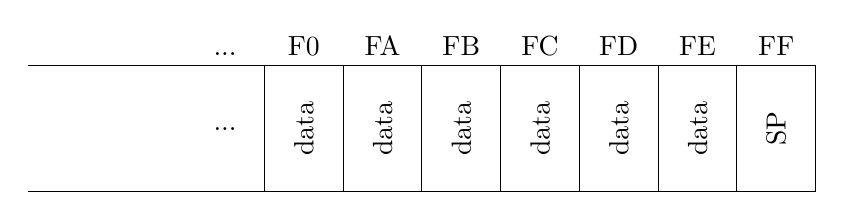
\begin{tikzpicture}
		\draw [-] (-10, 0) -- (0, 0) -- (0, 1.6) -- (-10, 1.6);
		\draw [-] (-1, 0) -- (-1, 1.6);
		\draw [-] (-2, 0) -- (-2, 1.6);
		\draw [-] (-3, 0) -- (-3, 1.6);
		\draw [-] (-4, 0) -- (-4, 1.6);
		\draw [-] (-5, 0) -- (-5, 1.6);
		\draw [-] (-6, 0) -- (-6, 1.6);
		\draw [-] (-7, 0) -- (-7, 1.6);
        \node[rotate=90] at (-0.5, 0.8) {SP};
        \node[rotate=90] at (-1.5, 0.8) {data};
        \node[rotate=90] at (-2.5, 0.8) {data};
        \node[rotate=90] at (-3.5, 0.8) {data};
        \node[rotate=90] at (-4.5, 0.8) {data};
        \node[rotate=90] at (-5.5, 0.8) {data};
        \node[rotate=90] at (-6.5, 0.8) {data};
        \node[above] at (-0.5, 1.6) {FF};
        \node[above] at (-1.5, 1.6) {FE};
        \node[above] at (-2.5, 1.6) {FD};
        \node[above] at (-3.5, 1.6) {FC};
        \node[above] at (-4.5, 1.6) {FB};
        \node[above] at (-5.5, 1.6) {FA};
        \node[above] at (-6.5, 1.6) {F0};
        \node at (-7.5, 0.8) {...};
        \node[above] at (-7.5, 1.6) {...};
	\end{tikzpicture}
\end{figure}
本次实验在原指令集的基础上扩增了三条指令压栈指令PUSHS,存栈指针指令SSP,取栈指针指令LSP.同时复用了退栈指令POPS(INC).
\subsection{流水机指令格式}
\section{指令格式}
\begin{table}[htbp!]
    \centering
    \begin{tabular}{p{1.5cm}<{\centering}|p{2cm}<{\centering}|p{4cm}<{\centering}|p{3.5cm}<{\centering}|p{2cm}<{\centering}|p{2cm}<{\centering}}
        \multirow{2}*{名称}&\multirow{2}*{助记符}&\multirow{2}*{功能}&\multicolumn{3}{c}{指令格式}\\
        \cline{4-6}~ & ~ & ~ & IR7 IR6 IR5 IR4 &IR3 IR2 & IR1 IR0\\
        \hline
        加法 & ADD $R_d$ $R_s$ & $R_d \leftarrow R_d\text{ and } R_s$ & 0001 & $R_d$& $R_s$\\
        减法 & SUB $R_d$ $R_s$ & $R_d \leftarrow R_d \text{ minus } R_s$ & 0010 & $R_d$& $R_s$\\
        逻辑与 & AND $R_d$ $R_s$ & $R_d \leftarrow R_d \text{ and } R_s$ & 0011 & $R_d$& $R_s$\\
        加1 & INC $R_d$ & $R_d \leftarrow R_d \text{ and } 1$ & 0100 & $R_d$& XX\\
        取数 & LD $R_d$ [$R_s$] & $R_d \leftarrow [R_s]$ & 0101 & $R_d$& $R_s$\\

    \end{tabular}
\end{table}
\section{上机调试通用流程}
在每次实验之前,我们都会先做下面几个工作
\subsection{写寄存器(100)}
按照之前的指令流程进行指令操作.具体是:
\begin{enumerate}[\indent\indent 1]
	\item $\text{SWCBA}\leftarrow \text{0b100}$
	\item QD
	\item $R_0\leftarrow \text{0b10101010}(\text{0xA5})$
	\item QD
	\item $R_1\leftarrow \text{0b01010101}(\text{0x5A})$
	\item QD
	\item $R_2\leftarrow \text{0b10101010}(\text{0xA5})$
	\item QD
	\item $R_3\leftarrow \text{0b01010101}(\text{0x5A})$
	\item QD
	\item CLR
\end{enumerate}
\subsection{读寄存器(011)}
按照之前的指令流程进行指令操作.具体是:
\begin{enumerate}[\indent\indent 1]
	\item $\text{SWCBA}\leftarrow \text{0b011}$
	\item QD
	\item QD
	\item QD
	\item CLR
\end{enumerate}
如果读出$R_0,R_1,R_2,R_3$无问题,则寄存器信号是可靠的,DBUS,SBUS是可靠的.
\subsection{运行代码(000)}
在寄存器中写入$R_0\leftarrow \text{A5}, R_1\leftarrow \text{5A}, R_2\leftarrow \text{5B}$.
在存储器中写入指令
\begin{enumerate}[\indent\indent]
	\item ADD $R_0$ $R_1$, 0001 0001
	\item SUB $R_0$ $R_2$, 0010 0010
	\item SUB $R_1$ $R_2$, 0010 0110
	\item INC $R_0$, 0100 00XX
	\item STOP, 1110 XXXX
\end{enumerate}
检查结果$R_0 = \text{A5}, R_1 = \text{00}, R_2 = \text{5B}$.并且注意信号灯C,Z是否正常.从此可以看出ALU部分功能有效,C,Z标志有效.
\subsection{进一步执行其他代码}
至此,花费10分钟就可以初步相信箱子正常工作.\\
\indent 至此可以自己写其他指令测试其他指令是否有效.\\
\indent 这里展示其中一个检测栈指令有效性的代码.\\
\indent 在寄存器中写入$R_0\leftarrow \text{FA}, R_1\leftarrow \text{0C}, R_2\leftarrow \text{00}, R_2\leftarrow \text{55}$.\\
\indent 在存储器中写入指令:
\begin{enumerate}[\indent\indent]
	\item LSP, 1111 1111,
	\item PUSH $R_0$, 1100 1100,
	\item PUSH $R_1$, 1100 1101,
	\item SSP, 1011 1111
\end{enumerate}
检查存储器[FF] = FC, [FE] = FA, [FD] = 0C.检查$R_3=\text{FC}$.
\section{调试过程中的问题及讨论}
\subsection{代码无法导入箱子或者代码导入箱子以后测试程序仍然发生以前的问题}
这里暂且不考虑箱子信号的问题,具体原因可能有几个.
\begin{enumerate}[1]
	\item 串口损坏,导致写入箱子失败.
	\item 箱子板子识别损坏,导致电脑无法针对这个芯片写入程序.
	\item 电脑只会写入一个文件项目,如果在测试过程中换了文件,需要在写入前确认是否写入目标文件是否是自己想要的文件.
\end{enumerate}
\subsection{程序运行失败}
考虑信号问题
\begin{enumerate}[1]
	\item dp单拍未设定,导致程序直接运行到stop或者因为没有stop,在主存中持续运行.(表现行为是,程序一闪而过或者W1,W2,W3信号灯在同一时间发亮.)
	\item PCINC信号失效.(表现行为是PCINC信号灯不亮或者PCINC信号灯已经亮但内部电路失效,这种情况对于所有信号都是一样的,所以下略,只说明失效时的电路行为.此时PC灯未能自增)
	\item LIR信号失效(此时IR灯始终为初始状态).
	\item AR损坏,表现行为是计算预期地址和实际显示AR不一致.
	\item 信号冲突,并行信号如果有先后关系,则有很大概率失败,比如STOP/SST0.
	\item 当上述情况均为发生,应当考虑是否是程序代码有问题.
\end{enumerate}
\subsection{隐含敏感指令问题}
\begin{enumerate}
	\item 
\end{enumerate}
\section{设计调试小结}
\subsection{向阳曦的总结}
在调试硬件及其编程语言时,一定要注意硬件的不可靠性.\\
\indent 所以在所有测试开始之前一定要先做如下步骤:
\begin{enumerate}[\indent \indent 1]
	\item 测试数据通路是否有问题.这个可以使用读写寄存器判断,可以迅速推断问题.
	\item 如果已知之前有程序能够运行,先跑这两个简单指令的程序,如果无错,则推测是在程序指令中有信号错误.
	\item 根据已知信号无错,缩小以后的信号调试错误推测范围.最后能够确定该系统在独立情况下信号无错的结论.
	\item 根据程序使用的信号无错,推断程序的指令是否有问题.
	\item 根据程序的指令是否在表面上有问题,推测是否是深层逻辑问题.
\end{enumerate}
\indent\indent 得到这些经验还是要拜托实验室里成群不能用的箱子.里面的箱子坏的各有特色,不带重样,因此积累了大量经验.
关于程序部分,我和张研究了一会如何设计指令.从x86中挑选了大约十条指令,并设计了指令格式.等到开始编写时,才发现$\text{IR}_{3210}$虽然和$\text{SEL}_{3210}$的值相同,但是因为$\text{SEL}_{3210}$只能用于控制台读写寄存器的输出,所以$\text{IR}_{3210}$是无法读出的.未果,寻弃.\\
\indent 最终我们选择完整地把PUSHS,POPS一整套栈操作完成.但是按照正常流程PUSHS,应当是:\\
\indent \indent 1.得到SP;2.写入SP;3.SP下推.
\\ 但是SP在硬件中没有专门存储器,寄存器只有4个,占用其中一个的代价太高.如果每次从主存取,周期占用太多.因此设计了新的LSP和SSP.采用一般数据库prepare的思路.这时又遇到问题了.LSP的流程应当是:\\
\indent \indent 1.得到SP在主存地址;2.读入SP到寄存器中.\\
\indent 这里我们如何去硬编码SP的地址是个问题.\\
\indent 深思熟虑以后.我们将SP地址从寄存挪到主存,再到最后敲定一个特殊的地址.我们选择了FF.因为这个根据任意8位2进制数字$A$或上$\overline{A}$永远等于FF.所以限定$A,B$为相同寄存器,就能在一个周期得到硬编码的FF写入AR.最后实际的设计为:\\
\indent \indent 1.要求A,B选择的寄存器一致;2.第一个周期将$A|\overline{B}$送入AR.3.取出FF上的值到$A$寄存器上.\\
\indent 这样只需要额外一条指令就能临时得到$SP$,额外另一条指令就能存储$SP$.\\
\indent 最后,我们将栈设计为向下生长,将POPS合并到INC SP中.又节约了一条指令空间,将这个指令编码给了另一个指令MOV.
\subsection{张逸群的总结}
课程设计让我对计算机组成原理有了更深刻的了解.\\
\indent 就课程设计的要求来说,流水机器和非流水机的差别不大,无非是什么时候取指令的问题.非流水机需要一个额外的时钟来取值,由于TEC8最多只有3个时钟,也就是说其他操作要在2个时钟内完成,这个给设计带来了很大的不便.流水机在执行的时候顺便取指令,这样能节约出来一个周期.\\
\indent 设计的时候主要考虑每个信号什么时候应该为1,然后在进程里面相应的地方给输出赋值即可.然后VDHL的进程会在敏感参数表发生改变的时候唤醒.所以不能直接在进程里面修改敏感信号,要新建一个SIGNAL记录有没有修改输出,然后在每个时钟的下降沿修改输出,这样就不会一直唤醒自己了.\\
\indent 还有个问题是指令的问题,由于TEC8的模式是前四位是指令,后四位是参数,由于后四位只能读入不能输出,所以参数必须要手动给出,而且用不了立即数的形式,这样的结果是一些原本很简单的操作会变得非常麻烦,需要用寄存器中转一下.有些原本可以隐式给出的参数也必须需要手动给出,不过有个例外是FF,这个可以通过ALU算出来,因为$A|(!A)=FF$,同理$A\&(!A)=0$,也可以不用手动给出.不过这样的代价是浪费了一个周期来计算隐式给出的参数.\\
\indent 剩下的问题都不是太多了,按照求出来的表达式写一下就可以了.
\end{document}